% Monografia para Projeto de Fim de Curso - Felipe T. C. Ribeiro
%-----------------------------------------------------------


%---------------Inicializa��o de pacotes--------------------

\documentclass[12pt,a4paper,notitlepage,twoside]{book}
\usepackage{times}

\usepackage{graphicx}
\usepackage[latin1]{inputenc}
\usepackage[brazil]{babel}
\usepackage[T1]{fontenc}
\usepackage{amsmath}
\usepackage{amsthm,amsfonts}
\usepackage{color}
%\usepackage{hyperref}
\usepackage[square,numbers]{natbib}
\bibliographystyle{abbrvnat}
\usepackage{abntex2abrev}
\usepackage{url}
\urlstyle{same}
%\usepackage[
%backend=biber,
%style=alphabetic,
%sorting=ynt
%]{biblatex}
%\addbibresource{references.bib}

\usepackage[a4paper,top=30mm,bottom=30mm,inner=30mm,outer=25mm,headheight=7mm,headsep=6mm,footskip=7mm]{geometry}
%\usepackage{epsfig}
%\usepackage{latexsym}
%\usepackage{float}
%\usepackage{quotes}
%\pagestyle {plain}
\makeindex

\def\baselinestretch{1.0}

%---------------In�cio do documento-------------------------

\begin{document}

\begin{titlepage}
\begin{center}
{\large Universidade Federal de Minas Gerais\\
Escola de Engenharia \\
Curso de Gradua��o em Engenharia de Controle e Automa��o\\}

\vspace{6cm}
{\bf\Large Aplica��o para c�lculo de indicadores de performance de malhas de controle de processos industriais\vspace{0.2cm}

%Segunda Linha do T�tulo, se Houver}
%\vspace{4cm}

%\hspace{0.3\textwidth} \parbox{0.65\textwidth}
{\large Felipe T. C. Ribeiro}
\vspace{2cm}  
   
\vspace{2cm}          
%\hspace{0.3\textwidth} 
{\large Orientador: Prof. Frederico Gualberto Ferreira Coelho.}\\
{\large Supervisor: Eng. Bernardo William Cafiero Viana}

\vfill
%\hspace{0.3\textwidth} 
{\large Belo Horizonte, Dezembro de 2020 }
\end{center}

\end{titlepage}

\newpage
\clearpage
\thispagestyle{empty}


\begin{titlepage}

\centering
\textbf{Monografia}\\
\vspace{2cm}
\centering
\textbf{Aplica��o para c�lculo de indicadores de performance de malhas de controle de processos industriais}\\
\vspace{5cm} 

\parbox{1.0\textwidth} 
{\large 
Monografia submetida � banca examinadora
designada pelo Colegiado Did�tico do Curso de
Gradua��o em Engenharia de Controle e
Automa��o da Universidade Federal de Minas
Gerais, como parte dos requisitos para aprova��o na
disciplina Projeto Final de Curso II.}

\vspace{7cm} 
\centering
Belo Horizonte, Julho de 2014

\end{titlepage}

\clearpage
\thispagestyle{empty}
\cleardoublepage

\pagenumbering{roman}
%\addcontentsline{toc}{chapter}{Resumo}

\begin{center}
\huge{{\bf Resumo}}
\vspace{2cm}
\end{center}
 
O presente trabalho apresenta o processo de desenvolvimento de uma aplica��o para c�lculo de �ndices de performance de malhas de controle, implantada em conjunto a um sistema CPM, sigla do ingl�s para \textit{Controller Performance Monitoring}, que recebe o nome de LOOP, desenvolvido pela empresa \textit{IHM Stefanini}. O sistema em quest�o � utilizado por um conjunto de diferentes clientes da ind�stria nacional como ferramenta para acompanhamento e metrifica��o dos estados de suas malhas de controle. Para tais avalia��es � comum a utiliza��o de �ndices de performance, que traduzem a n�meros, o desempenho de um sistema de controle. Nesse ponto entra a aplica��o alvo desse projeto, que recebe o nome de Kpi-Executor. O Kpi-Executor foi constru�do para a realiza��o dos c�lculos dos �ndices de performance, do ingl�s \textit{Key Performance Indicators}, abreviado por KPIs, que s�o parte essencial do sistema LOOP. � desejado que esta aplica��o se integre sem problemas ao sistema existente, em substitui��o a uma anterior com fun��o semelhante, tendo sua execu��o realizada a cada hora, gerando assim os valores desses �ndices utilizados. Nessa monografia ser�o detalhados o processo de desenvolvimento desse software, al�m da concep��o te�rica dos �ndices de performance os utilizados pelo sistema: Tempo em modo normal, Tempo sem satura��o, Erro m�dio aceit�vel e Nota global. Como resultados s�o apresentados documenta��o de regras de neg�cio gerada, a estrutura de logs para melhoria na etapa de manuten��o e evolu��o do software, al�m da estabiliza��o e repetibilidade obtidas pelo Kpi-Executor. 
 
%\begin{sloppypar}
%Este novo par�grafo serve para mostrar que ao pular uma ou mais linhas no texto do arquivo .tex, o \TeX\ entende que voc� est� iniciando outro par�grafo. O comando sloppypar for�a o texto a n�o ultrapassar as margens. S� deve ser usado se este problema ocorrer.
%\end{sloppypar}

 
\clearpage
\thispagestyle{empty}
\cleardoublepage


%\addcontentsline{toc}{chapter}{Agradecimentos}

\begin{center}
\huge{{\bf Agradecimentos}}
\vspace{4cm}
\end{center}

\begin{center}
	\begin{quotation}
		{\bf "Pra que amanh\~{a} n\~{a}o seja s\'{o} um ontem com um novo nome", Leandro}
	\end{quotation}
\end{center}



A Deus pela coragem e for\c{c}a concedida. \`{A} minha m\~{a}e, S\^{o}nia, pelo exemplo de for\c{c}a, resili\^{e}ncia e por todo apoio e ensinamento sobre jornadas. Ao meu pai por sua import\^{a}ncia no meu amadurecimento. \`{A}s minhas amigas e colegas de curso Lud, Manu e Pena que sabem exatamente o porque de estarem aqui. \`{A} expans\~{a}o da minha fam\'{i}lia nas pessoas de Gutenberg, Lidiane, Let\'{i}cia e av\'{o}s. A todos os amigos de caminhada. Por fim, n\~{a}o menos importante, minha esposa, Larissa.


\begin{center}
	\begin{quotation}
		{\bf M\~{a}e! A favela venceu!}
	\end{quotation}
\end{center}

 
\clearpage
\thispagestyle{empty}
\cleardoublepage
\setcounter{tocdepth}{3}
\setcounter{secnumdepth}{3}
\tableofcontents
%\markboth{Conte�do}{Conte�do}

\clearpage
%\thispagestyle{empty}
%\cleardoublepage

% Normalmente, este arquivo s� cont�m isto.
%\listoffigures
\addcontentsline{toc}{chapter}{Lista de Figuras}
%\markboth{Lista de Figuras}{Lista de Figuras}

\clearpage
%\thispagestyle{empty}
%\cleardoublepage

% Normalmente, este arquivo s� cont�m isto.
%\listoftables
\addcontentsline{toc}{chapter}{Lista de Tabelas}
%\markboth{Lista de Tabelas}{Lista de Tabelas}

\clearpage
\thispagestyle{empty}
\cleardoublepage

% Normalmente, este arquivo s� cont�m isto.

\pagenumbering{arabic}
\setcounter{page}{1}
\chapter{Introdu��o}
\markright{\thechapter ~~~ Introdu��o}
%\label{intro}

%Se preferir, voc� pode apresentar este Cap�tulo antes da primeira Se��o, destacando os principais pontos que s�o abordados. %\cite{Raffo2008}

\section{Motiva��o e Justificativa}
%\markright{\thesection ~~~ Motiva��o}
%\label{motiva}

� incontest�vel a incessante busca do setor industrial pelo aumento do desempenho de suas unidades operacionais. Para que as empresas envolvidas nesse ramo possam se manter de forma significativa no mercado, � necess�ria a constante reavalia��o de seus processos, bem como de seus custos com energia, perdas e reprocessamento de material. Independentemente do setor de atua��o da ind�stria a ser avaliada, tais fatores possuem extrema import�ncia, devendo ser monitoradas, controladas e projetadas.

Para elucidar, tomemos como exemplo um processo de beneficiamento min�rio de ferro. Pode-se dividi-lo em: Britagem, peneiramento, moagem, classifica��o, concentra��o, espessamento e filtragem. Cada uma dessas etapas � composta por vari�veis a serem controladas de forma individual, como n�veis de tanque, temperatura e densidade de misturas, velocidades de motores, posi��es de v�lvulas, etc. Para estabelecer o comportamento desejado para tais processos, se faz necess�ria a aplica��o de estrat�gias de controle regulat�rio, avan�ado ou de outras naturezas. O conjunto composto por vari�vel a ser controlada e estrat�gia de controle utilizada � chamado de \textit{malha de controle}.

Implementado um sistema de controle, obt�m-se ent�o um processo minimamente adequado aos par�metros configurados para o contexto operacional escolhido. Entretanto, n�o menos importante que essa adequa��o t�cnica individual estabelecida por esse sistema, s�o os resultados e efeitos colaterais gerados naquela linha do processo,  bem como a avalia��o do conjunto em situa��es n�o previstas nas estrat�gias de controle. Dessa forma, o acompanhamento e metrifica��o do comportamento de sistemas de controle industriais ganha notabilidade dentro do setor industrial.


Para este monitoramento s�o utilizados softwares baseadis em CPM (\textit{Controller Performance Monitoring}). Eles possuem ferramental para an�lise temporal das malhas envolvidas,  avalia��o de par�metros de controladores, modelagem de processos e medi��o de KPIs (\textit{Key Performance Indicators}). Buscando este espa�o de mercado, a empresa IHM Stefanini desenvolveu o software LOOP, que se enquadra no tipo citado.

Nos �ltimos meses o time de desenvolvimento da empresa iniciou, juntamente ao time de analistas de controle que utilizam o sistema, um processo de identifica��o de pontos de melhoria do software LOOP, envolvendo quesitos de interface, regras de neg�cio, distribui��o de responsabilidades entre os m�dulos do sistema, arquitetura, integra��o de c�digo e documenta��o. Dentre os pontos n�o satisfat�rios listados pela equipe, o m�dulo respons�vel pelo c�lculo de KPIs foi apontado como cr�tico, sendo o primeiro a passar por mudan�as significativa. O projeto descrito por esta monografia aborda o processo de reconstru��o desse m�dulo.


\section{Objetivos do Projeto}
%\markright{\thesection ~~~ Objetivos}
%label{objetivos}

O objetivo do projeto � a constru��o de um m�dulo para c�lculo de �ndices de performance, utilizando-se de conhecimentos de Engenharia de software e desenvolvimento de sistemas. Como requisitos para aceita��o, o m�dulo deve possuir as seguintes caracter�sticas:
\begin{itemize}
	\item \textbf{Execu��o c�clica:} O c�lculo dos �ndices de performance � baseado em janelas de dados de uma hora. Dessa forma, ele deve possuir execu��o c�clica com um intervalos semelhantes;
	\item \textbf{Adequa��o � estrutura do sistema:} O m�dulo ser� utilizado para compor um sistema da empresa parceira, Ihm Stefanini, que j� possui outros m�dulos existentes. Assim � necess�rio que sejam respeitadas limita��es e conceitos do sistema como um todo;
	\item \textbf{Registro de falhas:} � necess�rio que o m�dulo apresente registros de falhas de cada uma das execu��es, n�o somente listando, mas tamb�m identificando quais tipos;
\end{itemize}




\section{Local de Realiza��o}
\label{sec:ihm}
%\markright{\thesection ~~~ A Empresa}
%\label{empresa}
O projeto de fim de curso foi desenvolvido em parceria com a empresa IHM Stefanini, no setor de Discovery da mesma, respons�vel pelo desenvolvimento, evolu��o e manuten��o da arquitetura e c�digo fonte dos sistemas ali desenvolvidos. O posto de trabalho variou entre as depend�ncias da empresa, e regime de \textit{home office}, conforme necess�rio.

A empresa realiza projetos e desenvolvimentos de Automa��o, El�trica, Montagem, bem como servi�os de otimiza��o de malhas, projetos de controle avan�ado e gest�o. Atua em diversas �reas da ind�stria, como Minera��o, Siderurgia \& Metais, Papel \& Celulose, e �leo \& G�s. 

A IHM Stefanini foi criada em 1994 inicialmente com o nome de IHM como uma integradora de sistemas, instrumenta��o, el�trica e TI Industrial. Com sua expans�o, passa a fazer parte do grupo Stefanini em 2015. A partir da� funda o departamento de inova��o e come�a a atuar na busca por tecnologias disruptivas e elabora��o de produtos digitais.

Atualmente a IHM Stefanini � dividida nos seguintes setores t�cnicos:
\begin{itemize}
	\item Departamento de TA;
	\item Departamento de TI Industrial;
	\item Departamento Intelig�ncia Industrial;
	\item Departamento de Discovery;
	\item Departamento de El�trica;
\end{itemize}

Este projeto foi desenvolvido no departamento de Discovery que tem como prop�sito a descoberta sistem�tica e estrutura��o de ofertas de alto valor agregado para a empresa. Subdividido em:
\begin{itemize}
	
	\item Produtos: Forma��o de produtos que resolvam problemas reais de clientes finais;
	\item Coder: Time respons�vel pelos softwares do setor. Estrutura, desenvolve e mant�m c�digos-fonte e infraestruturas das demandas do setor.
	
\end{itemize}



\section{Estrutura da Monografia}
%\markright{\thesection ~~~ Organiza��o do Trabalho}
\label{estruturaMono}

O trabalho est� estruturado em quatro cap�tulos, sendo o Cap�tulo 1 o conjunto contextualiza��o, relev�ncia e principais objetivos do projeto como um todo. O Cap�tulo 2 contempla apresenta��o e revis�o de conceitos b�sicos importantes para melhor entendimento do projeto. J� o Cap�tulo 3 traz informa��es sobre os recursos necess�rios, metodologia de desenvolvimento e implementa��o do projeto. No Cap�tulo 4, a apresenta��o e discuss�o de dados, bem como sugest�es e dificuldades a serem encontradas no projeto. Por fim, no Cap�tulo 5, s�o apresentadas as conclus�es obtidas no ap�s a elabora��o do projeto, e considera��es sobre poss�veis continuidades.

\chapter{Revis�o Liter�ria}
\markright{\thechapter ~~~ Revis�o Liter�ria}

Neste cap�tulo s�o apresentados os conceitos utilizados neste trabalho baseado na literatura. Na primeira se��o s�o abordadas defini��es processuais de desenvolvimento de um software. Na segunda s�o revisados termos de direcionamento t�cnico para este processo. Na terceira, conceitos de controle e automa��o importantes, enquanto, na quarta, trabalhos relevantes que abordam assuntos comuns ao projeto aqui relatado.

\section{Processo de Software}
%\markright{\thesection ~~~ Hist�rico}
%\label{hist}

Um processo de software � composto por um conjunto de atividades relacionadas que levam � produ��o de um produto de software \cite{engSw}. A utiliza��o deste conjunto de atividades auxilia no aumento da qualidade do produto desenvolvido, bem como sua manuten��o. De forma geral, um processo de software � composto de quatro grandes etapas:
\begin{itemize}
	\item \textbf{Especifica��o de Software:} Devem ser definidas as funcionalidades e limita��es de funcionamento do software a ser desenvolvido;
	\item \textbf{Projeto e Implementa��o do Software:} O software deve ser produzido buscando o atendimento das especifica��es;
	\item \textbf{Valida��o de software:} Deve ser validado para garantir o atendimento �s demandas solicitadas;
	\item \textbf{Evolu��o do Software:} Deve ser evolu�do e alterado conforme novas necessidades 
\end{itemize}

\subsection{Modelo em Cascata}

Existem diversos modelos de processo de software, dentre eles o modelo cascata, tamb�m conhecido como ciclo de vida de software. Este modelo consiste no encadeamento de suas etapas, tendo o in�cio de uma associado necessariamente ao final de outra. S�o elas:
\begin{itemize}
	\item \textbf{Defini��o de requisitos:} S�o definidas restri��es e metas do sistema por meio de entrevista com o usu�rio. Posteriormente s�o detalhadas a fim de se tornar especifica��o do sistema;
	\item \textbf{Projeto de Sistema e Software:} Etapa de defini��o de arquitetura geral do sistema. Envolve identifica��o e descri��o das abstra��es, m�dulos ou componentes, bem como o relacionamento entre eles;
	\item \textbf{Implementa��o:} O projeto de software � desenvolvido com seus conjuntos ou unidades de programas;
	\item \textbf{Integra��o e Testes de sistema:} Os m�dulos individuais do sistema elaborado s�o integrados e testados em conjunto, buscando assegurar o funcionamento conforme especificado;
	\item \textbf{Opera��o e manuten��o:} O sistema � colocado em uso. S�o efetuadas poss�veis corre��es de erros n�o descobertos em etapas anteriores. Expans�es e melhorias de implementa��o das unidades tamb�m podem ser realizadas nesta etapa.
\end{itemize}

Este modelo d� grande import�ncia � documenta��o gerada ao final de cada uma das etapas, geralmente amarrando o in�cio da etapa seguinte � aprova��o destes documentos. Ele tamb�m � consistente com outros modelos de processos de engenharia, tornando o processo mais vis�vel para o n�vel gerencial.

\subsection{Desenvolvimento �gil}

O desenvolvimento �gil se baseia na entrega de pequenos incrementos do produto de software, disponibilizando vers�es para o cliente, a cada per�odo de tempo especificado (em geral, duas ou tr�s semanas). Esse envolvimento do cliente durante o processo de constru��o possibilita o acompanhamento da evolu��o dos requisitos do sistema. Tem como outra forte caracter�stica a utiliza��o de conversas informa��es, minimiza��o da documenta��o, gerando mais responsividade do processo a poss�veis mudan�as nos requisitos do produto de software.


\begin{figure}[!htbp]
	\centering		
	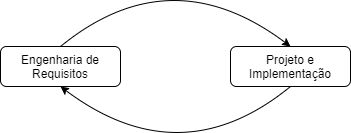
\includegraphics[width=0.5\textwidth]{RevisaoBibliografica/Images/MetodosAgeis.png}
	\caption{M�todos �geis}
	\label{fig:metAgeis}
\end{figure}


\section{Arquitetura de Software}
%talvez seja mais interessante utilizar o t�tulo "Modelagem de sistemas"
%\markright{\thesection ~~~ O Telefone}
%\label{telefone}

Arquitetura de Software � um conjunto de decis�es significativas sobre a
organiza��o de um sistema de software, a sele��o dos elementos estruturais e suas interfaces, a composi��o destes em subsistemas progressivamente maiores, bem como o estilo de arquitetura que orienta a organiza��o e intera��o dos m�dulos envolvidos. A defini��o da arquitetura de um software passa por etapas e conhecimentos pr�vios necess�rios para uma estrutura��o correta do mesmo \cite{umlBooch}.

\subsection{Modelagem orientada a Dados}
\label{sec:modSeq}
Modelos constru�dos sob o paradigma de orienta��o a dados trazem a sequ�ncia de a��es envolvidas no processamento daqueles dados, desde sua entrada, at� sua sa�da. Pode ser realizada atrav�s de um modelo de sequ�ncias\cite{umlBooch} destacando a movimenta��o dos dados daquele m�dulo ali representado. A figura \ref{fig:seqModel} traz um exemplo desse tipo de modelo.

\begin{figure}[!htbp]
	\centering		
	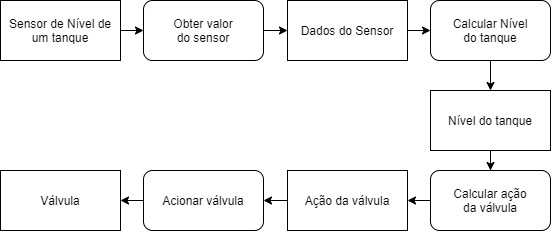
\includegraphics[width=0.75\textwidth]{RevisaoBibliografica/Images/modelSeq.png}
	\caption{Modelo de sequ�ncia}
	\label{fig:seqModel}
\end{figure}

\subsection{Arquitetura em Camadas}

Arquitetura que organiza o sistema em um grupo de camadas, onde cada uma delas oferece um conjunto de servi�os. Essa no��o de separa��o e independ�ncia � fundamental para que haja a possibilidade de altera��es localizadas, facilitando as etapas de manuten��o e sustenta��o do produto de software. A figura \ref{fig:arqCamadas} traz uma representa��o gen�rica deste tipo de arquitetura.

\begin{figure}[!htbp]
	\centering		
	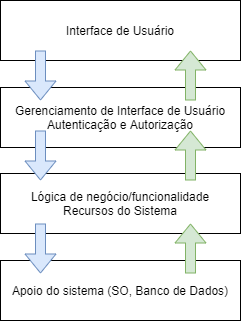
\includegraphics[width=0.4\textwidth]{RevisaoBibliografica/Images/ArqCamadas.png}
	\caption{Arquitetura gen�rica em camadas}
	\label{fig:arqCamadas}
\end{figure}

O relacionamento entre as camadas se d� de forma bem definida. Possui protocolos que indicam como a comunica��o entre elas se d�. Uma camada s� solicita servi�os � inferior, e somente fornece � superior.	Esse tipo de divis�o facilita e colabora para o processo de desenvolvimento incremental. Uma arquitetura deste tipo muito utilizada e conhecida � a \textit{MVC}, sigla do ingl�s para \textit{Model-View-Controller}.


\subsection{Orienta��o a Objetos}

O conceito de OO (Orienta��o a objetos) consiste na estrutura��o de um c�digo ou programa utilizando de abstra��es para conectar o espa�o do problema ao da solu��o. Os v�rios objetos constru�dos nessas abstra��es se relacionam atrav�s de comandos. Cada um desses objetos possui uma \textit{classifica��o} que o determina, chamada de \textit{classe}.

Para ficar claro como os objetos se relacionam, os conceitos que seguem s�o importantes	:
\begin{itemize}
	\item \textbf{Encapsulamento:} Estrat�gia utilizada para garantir que detalhes internos do funcionamento de uma classe. Dessa forma, o conhecimento sobre a implementa��o interna de uma classe � desnecess�ria do ponto de vista da inst�ncia daquela classe.;
	\item \textbf{Heran�a:} Quando uma classe pode ser um \textit{tipo} de uma outra classe, o conceito de heran�a pode ser aplicado. Se existe uma classe \textit{ve�culo} e se deseja construir uma representa��o \textit{motocicleta}, a segunda (classe filha) pode herdar caracter�sticas da primeira (classe pai), visto que \textit{bicicleta} � um tipo de \textit{ve�culo};
	\item \textbf{Polimorfismo:} � o princ�pio pelo qual duas ou mais classes derivadas de uma mesma classe pai podem invocar m�todos que t�m a mesma identifica��o (assinatura) mas comportamentos distintos, especializados para cada classe derivada, usando para tanto uma refer�ncia a um objeto do tipo da superclasse.;
\end{itemize}


\subsection{Modelo Relacional de Banco de Dados}

Banco de dados � uma mecanismo de armazenamento que permite persist�ncia de dados de uma aplica��o, programa ou produto de software. O modelo relacional busca o aumento da independ�ncia de dados nos sistemas. O Modelo relacional revelou-se ser o mais flex�vel e adequado ao solucionar os v�rios problemas que se colocam no n�vel da concep��o e implementa��o da base de dados. A estrutura fundamental do modelo
relacional � a rela��o. Ela � constitu�da por um ou mais atributos que traduzem o tipo de dados a armazenar \cite{intrBD}. 	

%TODO: Adicionar subsections sobre container, orquestradores(kubernetes) e imagens (docker);

%\section{Conceitos de Processos industriais}
%TODODetalhar sobre a utiliza��o de KPIs para an�lise de processos industriais. Falar aqui tamb�m sobre PIMS;
%\section{Trabalhos Relacionados}
%TODO Falar sobre o trabalho que est� no zotero sobre cria��o de aplica��o, depois falar sobre o artigo de kpis e partir pra ideia de ter um pouco de cada como refer�ncias;


\clearpage

%\chapter{Descri��o do Processo}

Se desejar, uma vis�o geral do Cap�tulo pode ser colocada antes da primeira Se��o. Este � o cap�tulo de descri��o do processo e formula��o do problema. Tendo em vista que se trata de uma monografia de engenharia de controle e automa��o, em muitos casos, � fundamental a apresenta��o dos sensores e atuadores do processo.


\section{Processo de Fazer Alguma Coisa}
\markright{\thesection ~~~ Hist�rico}
\label{hist}

...


\section{Instrumenta��o do Processo}
\markright{\thesection ~~~ O Telefone}
\label{telefone}



Continua ...


\section{Resumo do Cap�tulo}

N�o termine de forma abrupta.



\clearpage

\chapter{Materiais e M�todos}
\markright{\thechapter ~~~ Metodologia}
Neste cap�tulo s�o descritos os recursos de hardware e software necess�rios para o desenvolvimento deste projeto. S�o listados IDE utilizada para desenvolvimento, arquitetura existente a consumir dados da aplica��o e escolha de algoritmos de c�lculo de KPIs. Tamb�m s�o apresentados os processos de desenvolvimento de software utilizados e funcionamento da equipe dentro da qual foi o projeto foi constru�do.

\section{Descri��o de Componentes}

Esta se��o apresenta a arquitetura existente que receber� a aplica��o desenvolvida, o Kpi-Executor, bem como os recursos de hardware e software utilizados no seu desenvolvimento.

\subsection{Software}

\subsubsection{IDE, Linguagem e Banco de Dados}

Para o desenvolvimento da aplica��o foi escolhida a linguagem \textit{Python} \cite{pyPage}, em sua vers�o $3.8$, devido a seu car�ter de alto n�vel e sua grande gama de bibliotecas dispon�veis. Para a codifica��o foi escolhida a IDE \textit{Visual Studio Code} \cite{vscodePage}, devido � sua multiplicidade de extens�es e tamb�m por j� ser amplamente utilizada pela comunidade de desenvolvedores de software.

Ambas, linguagem e IDE, tem caracter�stica \textit{opensource}, sendo ativamente utilizadas e exploradas dia a dia por sua ampla comunidade, al�m de terem seus m�dulos e extens�es gratuitos.

Quanto ao armazenamento dos dados, foi utilizada uma estrutura relacional de banco de dados, considerando sua praticidade, bem como a estrutura existente descrita nas pr�ximas se��es. Foi utilizada uma inst�ncia de um banco de dados \textit{PostgresSQL} \cite{postgresPage} , uma ferramenta gratuita para a persist�ncia dos dados gerados pela aplica��o.

\subsubsection{Orquestradores e Containers}

Como a aplica��o desenvolvida foi acoplada a um sistema existente, foi necess�rio que ela respeitasse o conjunto anteriormente elaborado, bem como se adequasse � arquitetura em nuvem \cite{cloudComp} j� em funcionamento. Para tal, essa aplica��o deveria possuir certo encapsulamento.

Uma forma amplamente utilizada para o encapsulamento e execu��o de aplica��es de grande porte � o formato de \textit{containers}. � uma abordagem de desenvolvimento de software onde um servi�o ou aplicativo � empacotado com suas depend�ncias e configura��es \cite{containerIntr}. Dessa forma, s�o facilitados os processos de Testes de unidade e integra��o \cite{engSw}, bem como etapas de evolu��o \cite{engSw} e versionamento daquele conjunto. Para o processo de constru��o de \textit{container} do m�dulo \textit{Kpi-Executor} foi utilizada a plataforma \textit{Docker} \cite{dockerPage}, gerando uma imagem de um SO (Sistema Operacional) Linux contendo as depend�ncias e instala��es necess�rias para a execu��o do \textit{Kpi-Executor}.

Uma vez empacotada a aplica��o, � necess�rio utilizar uma ferramenta para operar esse pacote, o executando sempre que necess�rio. Esta utilidade � chamada de \textit{orquestrador}. A ferramenta deste tipo utilizada foi o \textit{Kubernetes} \cite{kubePage}. Este tipo de ferramenta possibilita a automa��o de opera��es \textit{containers}, como implanta��es ou atualiza��es das aplica��es, o gerenciamento de servi�os de forma declarativa garantindo a repetibilidade do sistema, a separa��o de \textit{containers} em diferentes \textit{hosts}, bem como a verifica��o de integridade e autorrecupera��o das aplica��es \cite{whatKube}.


\subsection{Estrutura Existente}

A aplica��o constru�da funcionar� como um m�dulo de um sistema de CPM existente chamado LOOP. Ele � composto por um conjunto de m�dulos, cada um com sua responsabilidade bem definida. A figura \ref{fig:arqLoop} traz o esquema arquitetural do sistema, bem como o relacionamento entre os m�dulos.

\begin{figure}[!htbp]
	\centering		
	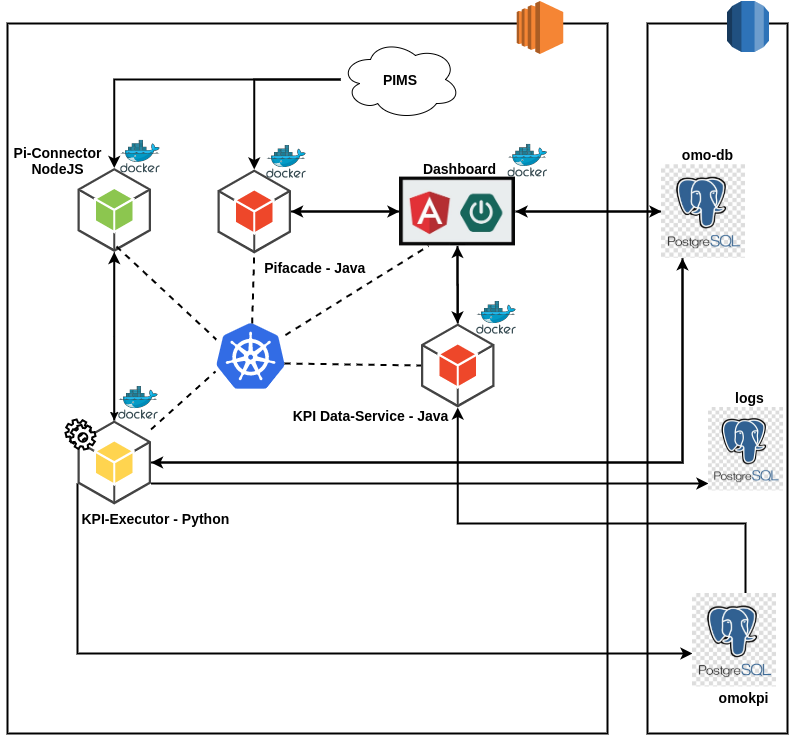
\includegraphics[width=10cm]{Metodologia/Figuras/arquitetura-omo.png}
	\caption{Arquitetura Loop}
	\label{fig:arqLoop}
\end{figure}

Neste esquema s�o identificadas as linguagens e tecnologias de cada m�dulo. S�o eles:

\begin{itemize}
	\item \textbf{Dashboard:} Aplica��o web acess�vel ao usu�rio do sistema CPM LOOP composta por um \textit{backend} em \textit{Spring Boot} \cite{springBootPage} e \textit{frontend} em \textit{AngularJS} \cite{angularJSPage};
	\item \textbf{Bancos de Dados:} S�o tr�s inst�ncias de banco de dados do sistema. A nomeada como \textit{omo-db} carrega as informa��es de cadastro e configura��o das entidades do LOOP. A nomeada \textit{omokpi} armazena os dados calculados pelo Kpi-Executor, enquanto a \textit{logs} registra os logs de funcionamento da aplica��o de c�lculos. Todas as inst�ncias s�o do tipo PostgreSQL \cite{postgresPage};
	\item \textbf{Data-Service:} M�dulo do tipo API constru�do em \textit{Spring Boot} \cite{springBootPage} respons�vel por prover dados registrados no banco \textit{omokpi} � aplica��o web \textit{Dashboard}. Formata pesquisa e retorna dados sob demanda;
	\item \textbf{PIMS:} Um sistema PIMS da \textit{OsiSoft} chamado \textit{PI System} \cite{piPage}. Nele s�o armazenados os dados de processo dos clientes que utilizam o sistema LOOP. Estes dados s�o utilizados na realiza��o dos c�lculos (Kpi-Executor);
	\item \textbf{Pi-Facade:} M�dulo do tipo API constru�do em \textit{Spring Boot} \cite{springBootPage} respons�vel por prover dados registrados e cadastrar novas informa��es no PIMS sob demanda da aplica��o web \textit{Dashboard};
	\item \textbf{Pi-Connector:} M�dulo do tipo API constru�do em \textit{NodeJS} \cite{nodejsPage} respons�vel pelo fornecimento de dados registrados no PIMS � aplica��o de c�lculos (Kpi-Executor);
	\item \textbf{Kpi-Executor:} M�dulo desenvolvido descrito por esta monografia. Constru�do em \textit{Python 3.8} \cite{pyPage} e respons�vel por calcular os �ndices de performance (KPIs) do sistema LOOP. Opera de forma c�clica, realizando seus c�lculos a cada hora.
	
\end{itemize}


\newpage
\subsection{Hardware}
Para realiza��o do desenvolvimento do Kpi-Executor, foi necess�rio um notebook com 16Gb de mem�ria e processador intel i7. Tamb�m foi necess�rio um ambiente de Testes e valida��o semelhante ao de produ��o. S�o m�quinas hospedadas na \textit{Amazon Web Services} \cite{awsHome}.



\section{Metodologia}
%\markright{\thesection ~~~ Metodologia}

Para a constru��o dessa aplica��o foi utilizado o um processo de desenvolvimento de software composto por caracter�sticas de um cascata e um incremental \cite{engSw}. Como o projeto foi entendido como uma demanda associada ao fluxo de trabalho da equipe de Coder, descrita na se��o \ref{sec:ihm}, ele estava submetido a um fluxo de \textit{Kanban}, o que aponta para o quesito de entrega incremental quando associado ao sistema LOOP como um todo. Entretanto, como se tratava de uma tarefa n�o pequena, foram necess�rias etapas que coincidem com o processo cascata.
Neste cap�tulo ser�o listadas as etapas de projeto, desenvolvimento e testes do Kpi-Executor, bem como as escolhas relacionadas aos c�lculos por ele realizados.

\subsection{Processo de Desenvolvimento}

O processo de desenvolvimento da aplica��o iniciou-se com um escopo relativamente simples. Ela deveria realizar de forma c�clica um conjunto de c�lculos de �ndices de performance que s�o utilizados pelo sistema CPM LOOP, registr�-los em um banco de dados existente, com estrutura tamb�m definida, e possibilitar um rastreio de falhas no fluxo de c�lculos, identificando o qual tipo de erro, e em que momento este acontecera. Tendo essas informa��es, ainda foi eram necess�rias mais defini��es de casos espec�ficos n�o mapeados pela descri��o inicial. 

\subsubsection{Levantamento do Requisitos}

Considerando a necessidade de um mapeamento detalhado dos casos de c�lculo, foi realizado um processo de entrevista com o PO (\textit{Product Owner}) do sistema LOOP, a fim de elucidar o fluxo de c�lculo em seu estado ideal, poss�veis tratativas em casos n�o usuais e demais requisitos funcionais e n�o-funcionais. Deste levantamento, foi elaborado o diagrama de sequ�ncia (\ref{sec:modSeq}) tratando o fluxo a ser executado pelo Kpi-Executor, exibido na figura (\ref{fig:fluxoKpi}).

 \begin{figure}[!htbp]
 	\centering		
 	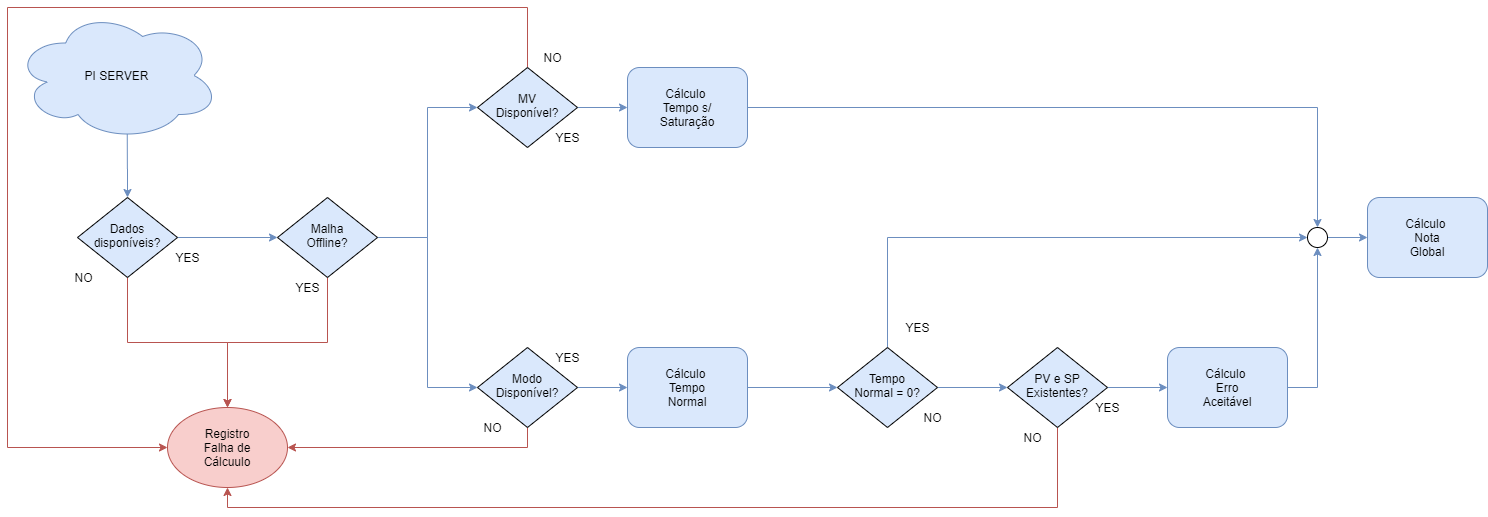
\includegraphics[width=14cm]{Metodologia/Figuras/fluxoKpiExecutor.png}
 	\caption{Diagrama de Sequ�ncia - Kpi-Executor}
 	\label{fig:fluxoKpi}
 \end{figure}
 
Ap�s constru��o deste diagrama de alto n�vel, foi realizada o nova reuni�o o validando como fluxo correto de c�lculos, incluindo as tratativas de casos espec�ficos. Assim p�de-se caminhar para a pr�xima etapa do processo.

\subsubsection{Projeto da Aplica��o}

Tendo requisitos funcionais e n�o-funcionais especificados, foi poss�vel ent�o o in�cio do projeto da aplica��o. Inicia-se pela defini��o arquitetural do m�dulo Kpi-Executor. Foi escolhida uma arquitetura em camadas (se��o \ref{sec:arqCamadas}) devido � familiaridade da equipe com o tipo de constru��o e a seu car�ter de atua��o sob demanda e persist�ncia em banco de dados. 

Para persist�ncia dos dados em banco, foi escolhida a tecnologia SQLAlchemy \cite{alchemyPage}, amplamente utilizada para acesso via Python a bancos de dados relacionais. Ela possibilita uma abordagem de orienta��o a objetos (se��o \ref{sec:seqOO}) em sua utiliza��o.

\subsubsection{Desenvolvimento da Aplica��o}

\paragraph {Classes auxiliares}
\label{sec:objDb}
Considerando a estrutura do sistema da empresa parceira (Loop) no momento do desenvolvimento do m�dulo tratado por essa monografia, era tido como de suma import�ncia a possibilidade de utiliza��o de diferentes bancos de dados relacionais, como Microfost SQL Server \cite{sqlServerHome} e PostgresSQL \cite{postgresPage}. Assim, foi necess�ria a utiliza��o da uma \textit{ORM} (Object Relacional Mapper) \cite{ORM} \textit{SQLAlchemy} \cite{alchemyPage}, possibilitando que o m�dulo em quest�o apresentasse caracter�sticas agn�sticas a banco de dados. Al�m da facilita��o no processo de substitui��o de bancos de dados, devido � objetifica��o das \textit{queries} adiciona seguran�a ao conjunto do sistema, impedindo tentativas de invas�o do tipo \textit{SQL Injection} \cite{SQLInjection}.

Uma vez levantados os pontos citados, foram utilizados os conceitos de orienta��o a objetos para o desenvolvimento (\ref{sec:seqOO}) para a elabora��o de duas classes que juntas tornariam o processo de constru��o das consultas e inser��es a banco de dados mais pr�ticas e robustas:

\begin{itemize}
	\item \textbf{Database:} Classe que contempla m�todos para conex�o e desconex�o com o banco de dados, bem como as informa��es de conex�o, como \textit{host}, nome do banco, usu�rio, senha e \textit{driver}. Seu uso consiste na representa��o de um banco de dados como um objeto. O \textit{SQLAlchemy} \cite{alchemyPage} faz gerenciamento autom�tico de m�ltiplas conex�es, possibilitando o instanciamento de diversos objetos dessa classe;
	\item \textbf{Repository:} Classe que contempla os m�todos b�sicos relacionados a consultas, inser��es, atualiza��es e dele��es. Seu uso consiste em t�-la como pai para cada nova classe com fun��es de acesso a dados. Possui um atributo do tipo \textit{Database} que aponta para o banco de dados a ser utilizado.
\end{itemize}

Uma vez elaboradas tais classes auxiliares, tem-se a etapa seguinte que contempla o conceito de divis�o de camadas (\ref{sec:arqCamadas}), novamente orienta��o a objetos (\ref{sec:seqOO}) e modelagem orientada a dados (\ref{sec:modSeq}).

\paragraph{Divis�o de Responsabilidades}

Considerando uma arquitetura de camadas, o Kpi-Executor foi modularizado dividindo as responsabilidades entre estes m�dulos. Foram separadas entre os componentes as tarefas de se consumir e escrever em diferentes bases de dados, operar o fluxo de c�lculos, registrar exce��es e falhas de c�lculo, etc. A figura \ref{fig:componentsKpi} traz o diagrama de componentes que descreve tal modulariza��o.

\begin{figure}[!htbp]
	\centering		
	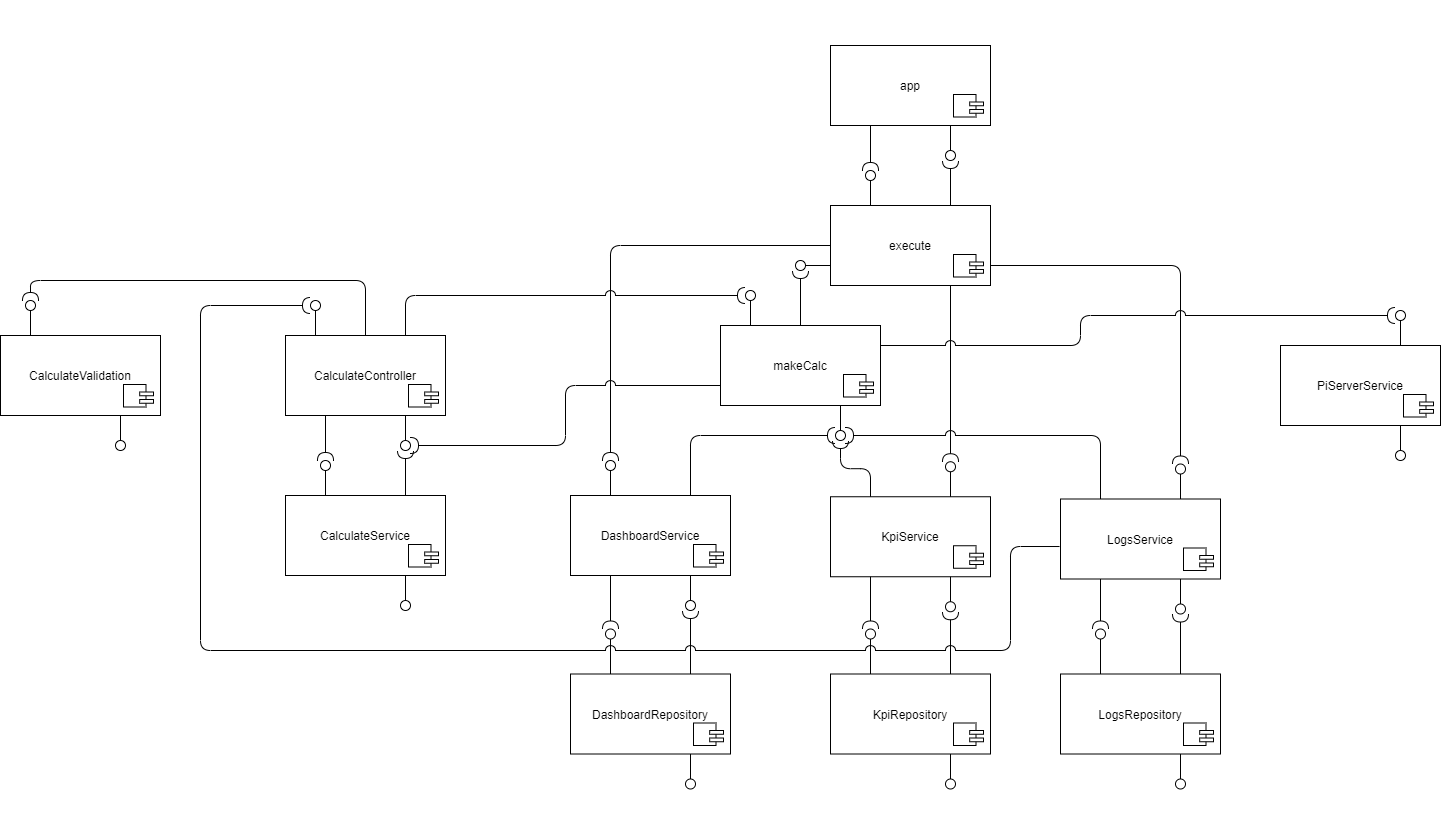
\includegraphics[width=14cm]{Metodologia/Figuras/kpiComponents.png}
	\caption{Diagrama de Componentes - Kpi-Executor}
	\label{fig:componentsKpi}
\end{figure}

Cada componente descrito no diagrama � composto por um arquivo independente em Python \cite{pyPage}, cada um com suas responsabilidades. 

\begin{itemize}
	\item \textbf{app:} Arquivo principal. Ele � o m�dulo invocado pelo orquestrador Kubernetes \cite{kubePage}. Respons�vel pela configura��o de logs de manuten��o e carregamento de vari�veis de ambiente do sistema, configurando a aplica��o para sua forma de execu��o local, em ambiente de valida��o ou produ��o;
	\item \textbf{execute:} Respons�vel por instanciar os objetos de banco de dados utilizados pelos pr�ximos componentes. Tamb�m invoca DashboardService para montar o objeto com os dados de cadastro para as etapas de c�lculos de KPIs;
	\item \textbf{makeCalc:} Opera o fluxo principal ta aplica��o. Percorre o objeto de dados de cadastro fornecido pelo componente \textit{execute} e solicitando, a cada itera��o, ao \textit{PiServerService} dados de processo cadastrados no PIMS, malha a malha;
	\item \textbf{DashboardService:} Possui regras de neg�cio relacionadas ao banco \textit{omo-db}. Formata os dados lidos e para inser��o neste banco. Tamb�m possui os m�todos para instanciar os objetos de banco de dados e para solicitar escrita no banco de dados;
	\item \textbf{DashboardRepository:} Possui os m�todos correspondentes �s queries de inser��o e consulta de dados em banco. Tem rela��o de heran�a \cite{engSw} com a classe \textit{Repository} (se��o \ref{sec:objDb});
	\item \textbf{PiServerService:} Contempla regras de neg�cio relacionadas � consulta de dados no PIMS. Formata e realiza requisi��es \textit{Http} para o m�dulo externo \textit{Pi-Connector} (figura \ref{fig:arqLoop}). Tamb�m possui rotinas para tratamento das respostas com os dados do PIMS;
	\item \textbf{KpiService:} Contempla as regras para formata��o de dados calculados para inser��o no banco \textit{omokpi};
	\item \textbf{LogsService:} Possui m�todos para conex�o com o banco de dados de logs de controle;
	\item \textbf{LogsRepository:} Possui m�todos relacionados a inser��o e leitura em dos logs em banco de dados. Tem rela��o de heran�a com a classe \textit{Repository} (se��o \ref{sec:objDb});
	\item \textbf{CalculateController:} Componente chave para o funcionamento da aplica��o. Contempla o fluxo descrito pelo levantamento de requisitos na figura \ref{fig:fluxoKpi}. Tamb�m invoca os m�dulos \textit{KpiService} e \textit{DashboardService} para registro de dados calculados e \textit{LogsService} para persist�ncia dos logs de controle;
	\item \textbf{CalculateService:} Possui os m�todos para a realiza��o dos c�lculos dos �ndices de performance. � invocado pelo \textit{calculateController};
	\item \textbf{CalculateValidation:} Possui m�todos auxiliares para a valida��o do fluxo de c�lculos. � invocado pelo \textit{CalulateController};
	
\end{itemize}

\paragraph{�ndices de Performance - KPIs}

\todo[inline]{Explicar os c�lculos realizados e citar a se��o (ainda n�o constru�da) da revis�o bibliogr�fica sobre os �ndices de performance.}

\paragraph{Registro de Logs de C�lculo}

\todo[inline]{Adicionar aqui o processo de estrutura��o dos logs de c�lculo em banco de dados. Associar esse processo ao fluxo da se��o de levantamento de requisitos.}


\subsubsection{Testes e Implanta��o}
\todo[inline]{Explicar etapas de teste com dados de cliente e valida��o de fluxo e resultados de c�lculos dos �ndices de performance}
\clearpage
%\chapter{Resultados}

Para a execu��o do projeto, algumas etapas de desenvolvimento tiveram de ser seguidas: familiariza��o com o sistema, estudo dos m�dulos envolvidos, leitura dos requisitos, elabora��o de documento descrevendo todo o processo de implementa��o e relacionamento com os diversos m�dulos, implementa��o e testes.

\section{Atividades do Projeto}
\markright{\thesection ~~~ Metodologia}
\label{metodo3}

\section {Requisitos do Sistema}
\markright{\thesection ~~~ Requisitos}
\label{req}






\begin{figure}[htbp]
\centering
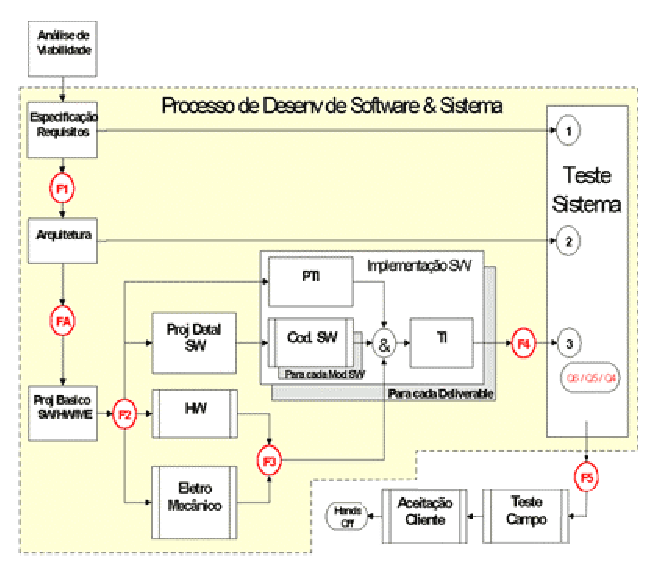
\includegraphics[scale=1.2]{Resultados/Figuras/ciclodesenvolvimento.eps}
\caption{Ciclo de desenvolvimento de um projeto}
\label{CicloDesenvolvimento}
\end{figure}

Para referenciar a Figura \ref{CicloDesenvolvimento}, veja arquivo .tex.



Aqui come�a uma sub-se��o.


\section{Desenvolvimeto e Implementa��o}

Aqui come�a outra se��o.

Para inserir a tabela abaixo, veja arquivo .tex.

\begin{table}
\centering
\begin{tabular}{|l|l|}\hline
		1.Uso do servi�o & Para o assinante rastrear uma chamada, ele dever� tirar\\ 
										 & o telefone do gancho, esperar pelo tom de discagem e ent�o \\
										 & discar o c�digo de acesso ao servi�o. \\ \hline
		2.Processamento  & Caso o assinante tenha acesso ao servi�o SRUC, ele dever�  \\			
		  do servi�o 		 & ouvir um an�ncio, ao discar o c�digo de acesso, explicando \\
									   & que o servi�o SRUC foi acessado. Dessa forma, se os dados \\
									   & a serem rastreados forem suficientes, o sistema dever� \\
									   & fornecer uma mensagem de confirma��o de \\
									   & servi�o realizado \\ \hline
		3. Ativa��o da   		& A ativa��o do servi�o somente ser� v�lida \\
			 �ltima chamada   & para a �ltima chamada recebida. \\ 
			 recebida				 	& \\ \hline
		4. Mais de uma   		& Se o assinante tentar ativar o servi�o para a mesma chamada \\
			 ativa��o para 	 	& ele dever� ouvir novamente o an�ncio de servi�o realizado, mas \\
			 a mesma chamada	& n�o ir� gravar os dados novamente \\ \hline
		5. N�mero privado 	& O sistema dever� mostrar o n�mero do assinante chamador \\
			 do assinante A  	& mesmo que este n�o possa ser mostrado. \\ \hline
		6. Chamadas  				& Para que o servi�o possa valer para chamadas intercentrais \\
			 intercentrais		& a central dever� utilizar a sinaliza��o SS7, e o n�mero do \\
												& assinante A ser� obtido pela mensagem IAM. \\ \hline
		7. Informa��es de 	& Um \textit{trace} do servi�o dever� possuir os seguintes itens:\\
			 um registro			& N�mero do assinante A \\
												& Hora da chamada recebida\\
												& Data da chamada recebida\\
												& N�mero do assinante B\\
												& Hora da solicita��o do servi�o\\
												& Data da solicita��o do servi�o\\
												& Dados sobre rota para chamadas intercentrais \\ \hline
		8. Tratamento para 	& Se um assinante discar o c�digo de acesso ao \\
		   assinante sem 		& servi�o, a central dever� fornecer tratamento padr�o \\
			 servi�o					& de acesso negado. \\ \hline
		9. Tipos de 				& A central deve permitir que o assinante com o servi�o \\
		   telefones				& possua tanto DTMF quando Dial Pulse \\ \hline
		10. Comandos do 		& O sistema supervis�rio conectado � central dever� \\
		    sistema 				& disponibilizar um  comando para que o operador possa  \\
		    supervis�rio		& descarregar o arquivo com os \textit{traces} das chamadas \\
		    								& para os diversos assinantes de uma central. \\
												& Um comando para visualizar os \textit{traces} tamb�m ser� necess�rio. \\ \hline
		\end{tabular}
	\caption{Requisitos do Servi�o SRUC}
	\label{tab:RequisitosDoServi�oSRUC}
\end{table}

Aqui voc� referencia a tabela: a Tabela \ref{tab:RequisitosDoServi�oSRUC} explicita os pontos mais relevantes na implementa��o do SRUC.

\section{Testes}

\section{Resumo do Cap�tulo}
\markright{\thesection ~~~ Metodologia}
\label{metodo4}
Esse cap�tulo pode ser dividido em duas partes $	f=ma $ blaba \cite{bel/00}
 
\begin{gather}
	f=ma\\
	x=2\\
\end{gather}

\begin{align}
	f=ma\\
	x=2\\
\end{align}

\begin{eqnarray}
	f=ma\\
	x=2\nonumber\\
\end{eqnarray}


\clearpage
%\chapter{Conclus�es}

\section{Considera��es Finais}

Aqui vai o texto da conclus�o.

\section{Propostas de Continuidade}


\clearpage


\addcontentsline{toc}{chapter}{Refer�ncias Bibliogr�ficas}
%\bibliographystyle{plainnat}
\begin{small}
%\bibliography{telefonia}%,library}
\bibliography{references}
%% Monografia para Projeto de Fim de Curso - Felipe T. C. Ribeiro
%-----------------------------------------------------------


%---------------Inicializa��o de pacotes--------------------

\documentclass[12pt,a4paper,notitlepage,twoside]{book}
\usepackage{times}

\usepackage{graphicx}
\usepackage[latin1]{inputenc}
\usepackage[brazil]{babel}
\usepackage[T1]{fontenc}
\usepackage{amsmath}
\usepackage{amsthm,amsfonts}
\usepackage{color}
%\usepackage{hyperref}
\usepackage{abntex2abrev}


\usepackage[a4paper,top=30mm,bottom=30mm,inner=30mm,outer=25mm,headheight=7mm,headsep=6mm,footskip=7mm]{geometry}
%\usepackage{epsfig}
%\usepackage{latexsym}
%\usepackage{float}
%\usepackage{quotes}
%\pagestyle {plain}

\makeindex

\def\baselinestretch{1.0}

%---------------In�cio do documento-------------------------

\begin{document}

%\begin{titlepage}
\begin{center}
{\large Universidade Federal de Minas Gerais\\
Escola de Engenharia \\
Curso de Gradua��o em Engenharia de Controle e Automa��o\\}

\vspace{6cm}
{\bf\Large Aplica��o para c�lculo de indicadores de performance de malhas de controle de processos industriais\vspace{0.2cm}

%Segunda Linha do T�tulo, se Houver}
%\vspace{4cm}

%\hspace{0.3\textwidth} \parbox{0.65\textwidth}
{\large Felipe T. C. Ribeiro}
\vspace{2cm}  
   
\vspace{2cm}          
%\hspace{0.3\textwidth} 
{\large Orientador: Prof. Frederico Gualberto Ferreira Coelho.}\\
{\large Supervisor: Eng. Bernardo William Cafiero Viana}

\vfill
%\hspace{0.3\textwidth} 
{\large Belo Horizonte, Dezembro de 2020 }
\end{center}

\end{titlepage}

\newpage
\clearpage
\thispagestyle{empty}


\begin{titlepage}

\centering
\textbf{Monografia}\\
\vspace{2cm}
\centering
\textbf{Aplica��o para c�lculo de indicadores de performance de malhas de controle de processos industriais}\\
\vspace{5cm} 

\parbox{1.0\textwidth} 
{\large 
Monografia submetida � banca examinadora
designada pelo Colegiado Did�tico do Curso de
Gradua��o em Engenharia de Controle e
Automa��o da Universidade Federal de Minas
Gerais, como parte dos requisitos para aprova��o na
disciplina Projeto Final de Curso II.}

\vspace{7cm} 
\centering
Belo Horizonte, Julho de 2014

\end{titlepage}

\clearpage
\thispagestyle{empty}
\cleardoublepage

\pagenumbering{roman}
%\addcontentsline{toc}{chapter}{Resumo}

\begin{center}
\huge{{\bf Resumo}}
\vspace{2cm}
\end{center}
 
O presente trabalho apresenta o processo de desenvolvimento de uma aplica��o para c�lculo de �ndices de performance de malhas de controle, implantada em conjunto a um sistema CPM, sigla do ingl�s para \textit{Controller Performance Monitoring}, que recebe o nome de LOOP, desenvolvido pela empresa \textit{IHM Stefanini}. O sistema em quest�o � utilizado por um conjunto de diferentes clientes da ind�stria nacional como ferramenta para acompanhamento e metrifica��o dos estados de suas malhas de controle. Para tais avalia��es � comum a utiliza��o de �ndices de performance, que traduzem a n�meros, o desempenho de um sistema de controle. Nesse ponto entra a aplica��o alvo desse projeto, que recebe o nome de Kpi-Executor. O Kpi-Executor foi constru�do para a realiza��o dos c�lculos dos �ndices de performance, do ingl�s \textit{Key Performance Indicators}, abreviado por KPIs, que s�o parte essencial do sistema LOOP. � desejado que esta aplica��o se integre sem problemas ao sistema existente, em substitui��o a uma anterior com fun��o semelhante, tendo sua execu��o realizada a cada hora, gerando assim os valores desses �ndices utilizados. Nessa monografia ser�o detalhados o processo de desenvolvimento desse software, al�m da concep��o te�rica dos �ndices de performance os utilizados pelo sistema: Tempo em modo normal, Tempo sem satura��o, Erro m�dio aceit�vel e Nota global. Como resultados s�o apresentados documenta��o de regras de neg�cio gerada, a estrutura de logs para melhoria na etapa de manuten��o e evolu��o do software, al�m da estabiliza��o e repetibilidade obtidas pelo Kpi-Executor. 
 
%\begin{sloppypar}
%Este novo par�grafo serve para mostrar que ao pular uma ou mais linhas no texto do arquivo .tex, o \TeX\ entende que voc� est� iniciando outro par�grafo. O comando sloppypar for�a o texto a n�o ultrapassar as margens. S� deve ser usado se este problema ocorrer.
%\end{sloppypar}

 
\clearpage
\thispagestyle{empty}
\cleardoublepage


%\addcontentsline{toc}{chapter}{Agradecimentos}

\begin{center}
\huge{{\bf Agradecimentos}}
\vspace{4cm}
\end{center}

\begin{center}
	\begin{quotation}
		{\bf "Pra que amanh\~{a} n\~{a}o seja s\'{o} um ontem com um novo nome", Leandro}
	\end{quotation}
\end{center}



A Deus pela coragem e for\c{c}a concedida. \`{A} minha m\~{a}e, S\^{o}nia, pelo exemplo de for\c{c}a, resili\^{e}ncia e por todo apoio e ensinamento sobre jornadas. Ao meu pai por sua import\^{a}ncia no meu amadurecimento. \`{A}s minhas amigas e colegas de curso Lud, Manu e Pena que sabem exatamente o porque de estarem aqui. \`{A} expans\~{a}o da minha fam\'{i}lia nas pessoas de Gutenberg, Lidiane, Let\'{i}cia e av\'{o}s. A todos os amigos de caminhada. Por fim, n\~{a}o menos importante, minha esposa, Larissa.


\begin{center}
	\begin{quotation}
		{\bf M\~{a}e! A favela venceu!}
	\end{quotation}
\end{center}

 
\clearpage
\thispagestyle{empty}
\cleardoublepage
%\setcounter{tocdepth}{3}
\setcounter{secnumdepth}{3}
\tableofcontents
%\markboth{Conte�do}{Conte�do}

\clearpage
%\thispagestyle{empty}
%\cleardoublepage

% Normalmente, este arquivo s� cont�m isto.
%\listoffigures
\addcontentsline{toc}{chapter}{Lista de Figuras}
%\markboth{Lista de Figuras}{Lista de Figuras}

\clearpage
%\thispagestyle{empty}
%\cleardoublepage

% Normalmente, este arquivo s� cont�m isto.
%\listoftables
\addcontentsline{toc}{chapter}{Lista de Tabelas}
%\markboth{Lista de Tabelas}{Lista de Tabelas}

\clearpage
\thispagestyle{empty}
\cleardoublepage

% Normalmente, este arquivo s� cont�m isto.

\pagenumbering{arabic}
\setcounter{page}{1}
\chapter{Introdu��o}
\markright{\thechapter ~~~ Introdu��o}
%\label{intro}

%Se preferir, voc� pode apresentar este Cap�tulo antes da primeira Se��o, destacando os principais pontos que s�o abordados. %\cite{Raffo2008}

\section{Motiva��o e Justificativa}
%\markright{\thesection ~~~ Motiva��o}
%\label{motiva}

� incontest�vel a incessante busca do setor industrial pelo aumento do desempenho de suas unidades operacionais. Para que as empresas envolvidas nesse ramo possam se manter de forma significativa no mercado, � necess�ria a constante reavalia��o de seus processos, bem como de seus custos com energia, perdas e reprocessamento de material. Independentemente do setor de atua��o da ind�stria a ser avaliada, tais fatores possuem extrema import�ncia, devendo ser monitoradas, controladas e projetadas.

Para elucidar, tomemos como exemplo um processo de beneficiamento min�rio de ferro. Pode-se dividi-lo em: Britagem, peneiramento, moagem, classifica��o, concentra��o, espessamento e filtragem. Cada uma dessas etapas � composta por vari�veis a serem controladas de forma individual, como n�veis de tanque, temperatura e densidade de misturas, velocidades de motores, posi��es de v�lvulas, etc. Para estabelecer o comportamento desejado para tais processos, se faz necess�ria a aplica��o de estrat�gias de controle regulat�rio, avan�ado ou de outras naturezas. O conjunto composto por vari�vel a ser controlada e estrat�gia de controle utilizada � chamado de \textit{malha de controle}.

Implementado um sistema de controle, obt�m-se ent�o um processo minimamente adequado aos par�metros configurados para o contexto operacional escolhido. Entretanto, n�o menos importante que essa adequa��o t�cnica individual estabelecida por esse sistema, s�o os resultados e efeitos colaterais gerados naquela linha do processo,  bem como a avalia��o do conjunto em situa��es n�o previstas nas estrat�gias de controle. Dessa forma, o acompanhamento e metrifica��o do comportamento de sistemas de controle industriais ganha notabilidade dentro do setor industrial.


Para este monitoramento s�o utilizados softwares baseadis em CPM (\textit{Controller Performance Monitoring}). Eles possuem ferramental para an�lise temporal das malhas envolvidas,  avalia��o de par�metros de controladores, modelagem de processos e medi��o de KPIs (\textit{Key Performance Indicators}). Buscando este espa�o de mercado, a empresa IHM Stefanini desenvolveu o software LOOP, que se enquadra no tipo citado.

Nos �ltimos meses o time de desenvolvimento da empresa iniciou, juntamente ao time de analistas de controle que utilizam o sistema, um processo de identifica��o de pontos de melhoria do software LOOP, envolvendo quesitos de interface, regras de neg�cio, distribui��o de responsabilidades entre os m�dulos do sistema, arquitetura, integra��o de c�digo e documenta��o. Dentre os pontos n�o satisfat�rios listados pela equipe, o m�dulo respons�vel pelo c�lculo de KPIs foi apontado como cr�tico, sendo o primeiro a passar por mudan�as significativa. O projeto descrito por esta monografia aborda o processo de reconstru��o desse m�dulo.


\section{Objetivos do Projeto}
%\markright{\thesection ~~~ Objetivos}
%label{objetivos}

O objetivo do projeto � a constru��o de um m�dulo para c�lculo de �ndices de performance, utilizando-se de conhecimentos de Engenharia de software e desenvolvimento de sistemas. Como requisitos para aceita��o, o m�dulo deve possuir as seguintes caracter�sticas:
\begin{itemize}
	\item \textbf{Execu��o c�clica:} O c�lculo dos �ndices de performance � baseado em janelas de dados de uma hora. Dessa forma, ele deve possuir execu��o c�clica com um intervalos semelhantes;
	\item \textbf{Adequa��o � estrutura do sistema:} O m�dulo ser� utilizado para compor um sistema da empresa parceira, Ihm Stefanini, que j� possui outros m�dulos existentes. Assim � necess�rio que sejam respeitadas limita��es e conceitos do sistema como um todo;
	\item \textbf{Registro de falhas:} � necess�rio que o m�dulo apresente registros de falhas de cada uma das execu��es, n�o somente listando, mas tamb�m identificando quais tipos;
\end{itemize}




\section{Local de Realiza��o}
\label{sec:ihm}
%\markright{\thesection ~~~ A Empresa}
%\label{empresa}
O projeto de fim de curso foi desenvolvido em parceria com a empresa IHM Stefanini, no setor de Discovery da mesma, respons�vel pelo desenvolvimento, evolu��o e manuten��o da arquitetura e c�digo fonte dos sistemas ali desenvolvidos. O posto de trabalho variou entre as depend�ncias da empresa, e regime de \textit{home office}, conforme necess�rio.

A empresa realiza projetos e desenvolvimentos de Automa��o, El�trica, Montagem, bem como servi�os de otimiza��o de malhas, projetos de controle avan�ado e gest�o. Atua em diversas �reas da ind�stria, como Minera��o, Siderurgia \& Metais, Papel \& Celulose, e �leo \& G�s. 

A IHM Stefanini foi criada em 1994 inicialmente com o nome de IHM como uma integradora de sistemas, instrumenta��o, el�trica e TI Industrial. Com sua expans�o, passa a fazer parte do grupo Stefanini em 2015. A partir da� funda o departamento de inova��o e come�a a atuar na busca por tecnologias disruptivas e elabora��o de produtos digitais.

Atualmente a IHM Stefanini � dividida nos seguintes setores t�cnicos:
\begin{itemize}
	\item Departamento de TA;
	\item Departamento de TI Industrial;
	\item Departamento Intelig�ncia Industrial;
	\item Departamento de Discovery;
	\item Departamento de El�trica;
\end{itemize}

Este projeto foi desenvolvido no departamento de Discovery que tem como prop�sito a descoberta sistem�tica e estrutura��o de ofertas de alto valor agregado para a empresa. Subdividido em:
\begin{itemize}
	
	\item Produtos: Forma��o de produtos que resolvam problemas reais de clientes finais;
	\item Coder: Time respons�vel pelos softwares do setor. Estrutura, desenvolve e mant�m c�digos-fonte e infraestruturas das demandas do setor.
	
\end{itemize}



\section{Estrutura da Monografia}
%\markright{\thesection ~~~ Organiza��o do Trabalho}
\label{estruturaMono}

O trabalho est� estruturado em quatro cap�tulos, sendo o Cap�tulo 1 o conjunto contextualiza��o, relev�ncia e principais objetivos do projeto como um todo. O Cap�tulo 2 contempla apresenta��o e revis�o de conceitos b�sicos importantes para melhor entendimento do projeto. J� o Cap�tulo 3 traz informa��es sobre os recursos necess�rios, metodologia de desenvolvimento e implementa��o do projeto. No Cap�tulo 4, a apresenta��o e discuss�o de dados, bem como sugest�es e dificuldades a serem encontradas no projeto. Por fim, no Cap�tulo 5, s�o apresentadas as conclus�es obtidas no ap�s a elabora��o do projeto, e considera��es sobre poss�veis continuidades.

%\chapter{Descri��o do Processo}

Se desejar, uma vis�o geral do Cap�tulo pode ser colocada antes da primeira Se��o. Este � o cap�tulo de descri��o do processo e formula��o do problema. Tendo em vista que se trata de uma monografia de engenharia de controle e automa��o, em muitos casos, � fundamental a apresenta��o dos sensores e atuadores do processo.


\section{Processo de Fazer Alguma Coisa}
\markright{\thesection ~~~ Hist�rico}
\label{hist}

...


\section{Instrumenta��o do Processo}
\markright{\thesection ~~~ O Telefone}
\label{telefone}



Continua ...


\section{Resumo do Cap�tulo}

N�o termine de forma abrupta.



\clearpage

%\chapter{Materiais e M�todos}
\markright{\thechapter ~~~ Metodologia}
Neste cap�tulo s�o descritos os recursos de hardware e software necess�rios para o desenvolvimento deste projeto. S�o listados IDE utilizada para desenvolvimento, arquitetura existente a consumir dados da aplica��o e escolha de algoritmos de c�lculo de KPIs. Tamb�m s�o apresentados os processos de desenvolvimento de software utilizados e funcionamento da equipe dentro da qual foi o projeto foi constru�do.

\section{Descri��o de Componentes}

Esta se��o apresenta a arquitetura existente que receber� a aplica��o desenvolvida, o Kpi-Executor, bem como os recursos de hardware e software utilizados no seu desenvolvimento.

\subsection{Software}

\subsubsection{IDE, Linguagem e Banco de Dados}

Para o desenvolvimento da aplica��o foi escolhida a linguagem \textit{Python} \cite{pyPage}, em sua vers�o $3.8$, devido a seu car�ter de alto n�vel e sua grande gama de bibliotecas dispon�veis. Para a codifica��o foi escolhida a IDE \textit{Visual Studio Code} \cite{vscodePage}, devido � sua multiplicidade de extens�es e tamb�m por j� ser amplamente utilizada pela comunidade de desenvolvedores de software.

Ambas, linguagem e IDE, tem caracter�stica \textit{opensource}, sendo ativamente utilizadas e exploradas dia a dia por sua ampla comunidade, al�m de terem seus m�dulos e extens�es gratuitos.

Quanto ao armazenamento dos dados, foi utilizada uma estrutura relacional de banco de dados, considerando sua praticidade, bem como a estrutura existente descrita nas pr�ximas se��es. Foi utilizada uma inst�ncia de um banco de dados \textit{PostgresSQL} \cite{postgresPage} , uma ferramenta gratuita para a persist�ncia dos dados gerados pela aplica��o.

\subsubsection{Orquestradores e Containers}

Como a aplica��o desenvolvida foi acoplada a um sistema existente, foi necess�rio que ela respeitasse o conjunto anteriormente elaborado, bem como se adequasse � arquitetura em nuvem \cite{cloudComp} j� em funcionamento. Para tal, essa aplica��o deveria possuir certo encapsulamento.

Uma forma amplamente utilizada para o encapsulamento e execu��o de aplica��es de grande porte � o formato de \textit{containers}. � uma abordagem de desenvolvimento de software onde um servi�o ou aplicativo � empacotado com suas depend�ncias e configura��es \cite{containerIntr}. Dessa forma, s�o facilitados os processos de Testes de unidade e integra��o \cite{engSw}, bem como etapas de evolu��o \cite{engSw} e versionamento daquele conjunto. Para o processo de constru��o de \textit{container} do m�dulo \textit{Kpi-Executor} foi utilizada a plataforma \textit{Docker} \cite{dockerPage}, gerando uma imagem de um SO (Sistema Operacional) Linux contendo as depend�ncias e instala��es necess�rias para a execu��o do \textit{Kpi-Executor}.

Uma vez empacotada a aplica��o, � necess�rio utilizar uma ferramenta para operar esse pacote, o executando sempre que necess�rio. Esta utilidade � chamada de \textit{orquestrador}. A ferramenta deste tipo utilizada foi o \textit{Kubernetes} \cite{kubePage}. Este tipo de ferramenta possibilita a automa��o de opera��es \textit{containers}, como implanta��es ou atualiza��es das aplica��es, o gerenciamento de servi�os de forma declarativa garantindo a repetibilidade do sistema, a separa��o de \textit{containers} em diferentes \textit{hosts}, bem como a verifica��o de integridade e autorrecupera��o das aplica��es \cite{whatKube}.


\subsection{Estrutura Existente}

A aplica��o constru�da funcionar� como um m�dulo de um sistema de CPM existente chamado LOOP. Ele � composto por um conjunto de m�dulos, cada um com sua responsabilidade bem definida. A figura \ref{fig:arqLoop} traz o esquema arquitetural do sistema, bem como o relacionamento entre os m�dulos.

\begin{figure}[!htbp]
	\centering		
	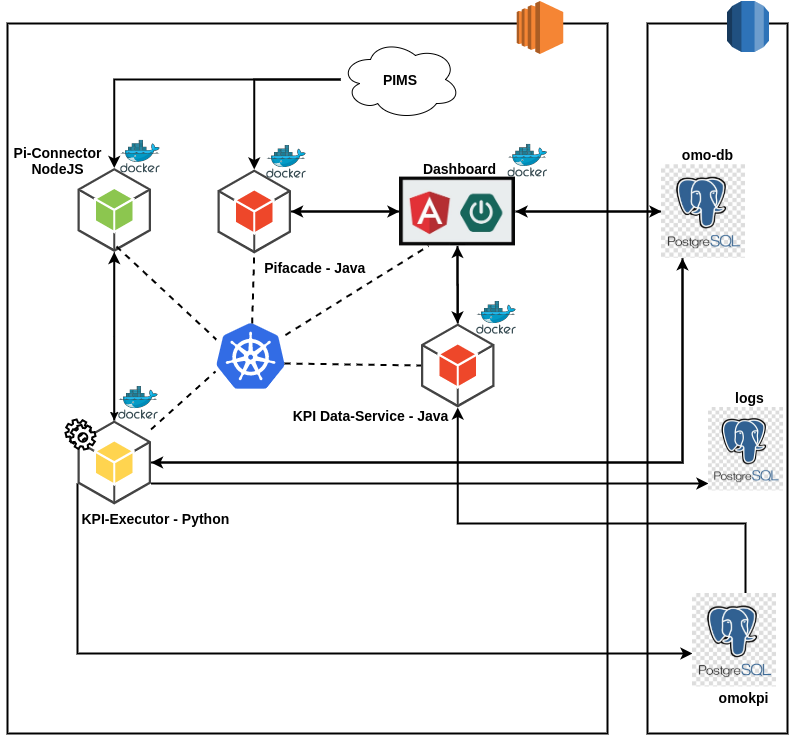
\includegraphics[width=10cm]{Metodologia/Figuras/arquitetura-omo.png}
	\caption{Arquitetura Loop}
	\label{fig:arqLoop}
\end{figure}

Neste esquema s�o identificadas as linguagens e tecnologias de cada m�dulo. S�o eles:

\begin{itemize}
	\item \textbf{Dashboard:} Aplica��o web acess�vel ao usu�rio do sistema CPM LOOP composta por um \textit{backend} em \textit{Spring Boot} \cite{springBootPage} e \textit{frontend} em \textit{AngularJS} \cite{angularJSPage};
	\item \textbf{Bancos de Dados:} S�o tr�s inst�ncias de banco de dados do sistema. A nomeada como \textit{omo-db} carrega as informa��es de cadastro e configura��o das entidades do LOOP. A nomeada \textit{omokpi} armazena os dados calculados pelo Kpi-Executor, enquanto a \textit{logs} registra os logs de funcionamento da aplica��o de c�lculos. Todas as inst�ncias s�o do tipo PostgreSQL \cite{postgresPage};
	\item \textbf{Data-Service:} M�dulo do tipo API constru�do em \textit{Spring Boot} \cite{springBootPage} respons�vel por prover dados registrados no banco \textit{omokpi} � aplica��o web \textit{Dashboard}. Formata pesquisa e retorna dados sob demanda;
	\item \textbf{PIMS:} Um sistema PIMS da \textit{OsiSoft} chamado \textit{PI System} \cite{piPage}. Nele s�o armazenados os dados de processo dos clientes que utilizam o sistema LOOP. Estes dados s�o utilizados na realiza��o dos c�lculos (Kpi-Executor);
	\item \textbf{Pi-Facade:} M�dulo do tipo API constru�do em \textit{Spring Boot} \cite{springBootPage} respons�vel por prover dados registrados e cadastrar novas informa��es no PIMS sob demanda da aplica��o web \textit{Dashboard};
	\item \textbf{Pi-Connector:} M�dulo do tipo API constru�do em \textit{NodeJS} \cite{nodejsPage} respons�vel pelo fornecimento de dados registrados no PIMS � aplica��o de c�lculos (Kpi-Executor);
	\item \textbf{Kpi-Executor:} M�dulo desenvolvido descrito por esta monografia. Constru�do em \textit{Python 3.8} \cite{pyPage} e respons�vel por calcular os �ndices de performance (KPIs) do sistema LOOP. Opera de forma c�clica, realizando seus c�lculos a cada hora.
	
\end{itemize}


\newpage
\subsection{Hardware}
Para realiza��o do desenvolvimento do Kpi-Executor, foi necess�rio um notebook com 16Gb de mem�ria e processador intel i7. Tamb�m foi necess�rio um ambiente de Testes e valida��o semelhante ao de produ��o. S�o m�quinas hospedadas na \textit{Amazon Web Services} \cite{awsHome}.



\section{Metodologia}
%\markright{\thesection ~~~ Metodologia}

Para a constru��o dessa aplica��o foi utilizado o um processo de desenvolvimento de software composto por caracter�sticas de um cascata e um incremental \cite{engSw}. Como o projeto foi entendido como uma demanda associada ao fluxo de trabalho da equipe de Coder, descrita na se��o \ref{sec:ihm}, ele estava submetido a um fluxo de \textit{Kanban}, o que aponta para o quesito de entrega incremental quando associado ao sistema LOOP como um todo. Entretanto, como se tratava de uma tarefa n�o pequena, foram necess�rias etapas que coincidem com o processo cascata.
Neste cap�tulo ser�o listadas as etapas de projeto, desenvolvimento e testes do Kpi-Executor, bem como as escolhas relacionadas aos c�lculos por ele realizados.

\subsection{Processo de Desenvolvimento}

O processo de desenvolvimento da aplica��o iniciou-se com um escopo relativamente simples. Ela deveria realizar de forma c�clica um conjunto de c�lculos de �ndices de performance que s�o utilizados pelo sistema CPM LOOP, registr�-los em um banco de dados existente, com estrutura tamb�m definida, e possibilitar um rastreio de falhas no fluxo de c�lculos, identificando o qual tipo de erro, e em que momento este acontecera. Tendo essas informa��es, ainda foi eram necess�rias mais defini��es de casos espec�ficos n�o mapeados pela descri��o inicial. 

\subsubsection{Levantamento do Requisitos}

Considerando a necessidade de um mapeamento detalhado dos casos de c�lculo, foi realizado um processo de entrevista com o PO (\textit{Product Owner}) do sistema LOOP, a fim de elucidar o fluxo de c�lculo em seu estado ideal, poss�veis tratativas em casos n�o usuais e demais requisitos funcionais e n�o-funcionais. Deste levantamento, foi elaborado o diagrama de sequ�ncia (\ref{sec:modSeq}) tratando o fluxo a ser executado pelo Kpi-Executor, exibido na figura (\ref{fig:fluxoKpi}).

 \begin{figure}[!htbp]
 	\centering		
 	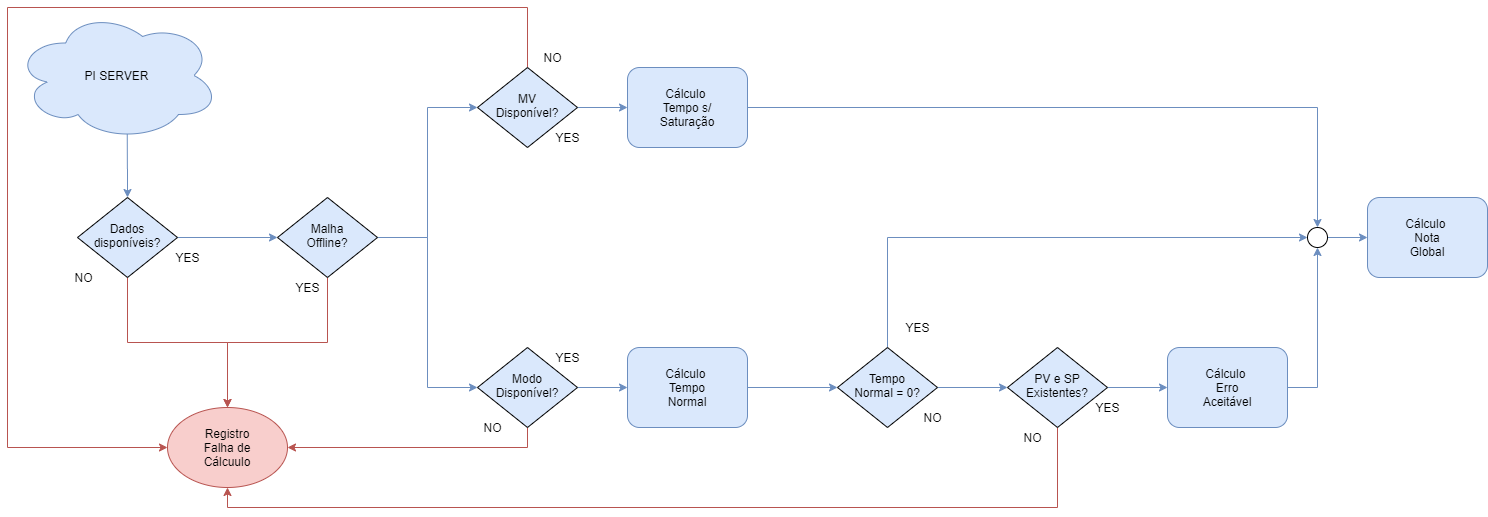
\includegraphics[width=14cm]{Metodologia/Figuras/fluxoKpiExecutor.png}
 	\caption{Diagrama de Sequ�ncia - Kpi-Executor}
 	\label{fig:fluxoKpi}
 \end{figure}
 
Ap�s constru��o deste diagrama de alto n�vel, foi realizada o nova reuni�o o validando como fluxo correto de c�lculos, incluindo as tratativas de casos espec�ficos. Assim p�de-se caminhar para a pr�xima etapa do processo.

\subsubsection{Projeto da Aplica��o}

Tendo requisitos funcionais e n�o-funcionais especificados, foi poss�vel ent�o o in�cio do projeto da aplica��o. Inicia-se pela defini��o arquitetural do m�dulo Kpi-Executor. Foi escolhida uma arquitetura em camadas (se��o \ref{sec:arqCamadas}) devido � familiaridade da equipe com o tipo de constru��o e a seu car�ter de atua��o sob demanda e persist�ncia em banco de dados. 

Para persist�ncia dos dados em banco, foi escolhida a tecnologia SQLAlchemy \cite{alchemyPage}, amplamente utilizada para acesso via Python a bancos de dados relacionais. Ela possibilita uma abordagem de orienta��o a objetos (se��o \ref{sec:seqOO}) em sua utiliza��o.

\subsubsection{Desenvolvimento da Aplica��o}

\paragraph {Classes auxiliares}
\label{sec:objDb}
Considerando a estrutura do sistema da empresa parceira (Loop) no momento do desenvolvimento do m�dulo tratado por essa monografia, era tido como de suma import�ncia a possibilidade de utiliza��o de diferentes bancos de dados relacionais, como Microfost SQL Server \cite{sqlServerHome} e PostgresSQL \cite{postgresPage}. Assim, foi necess�ria a utiliza��o da uma \textit{ORM} (Object Relacional Mapper) \cite{ORM} \textit{SQLAlchemy} \cite{alchemyPage}, possibilitando que o m�dulo em quest�o apresentasse caracter�sticas agn�sticas a banco de dados. Al�m da facilita��o no processo de substitui��o de bancos de dados, devido � objetifica��o das \textit{queries} adiciona seguran�a ao conjunto do sistema, impedindo tentativas de invas�o do tipo \textit{SQL Injection} \cite{SQLInjection}.

Uma vez levantados os pontos citados, foram utilizados os conceitos de orienta��o a objetos para o desenvolvimento (\ref{sec:seqOO}) para a elabora��o de duas classes que juntas tornariam o processo de constru��o das consultas e inser��es a banco de dados mais pr�ticas e robustas:

\begin{itemize}
	\item \textbf{Database:} Classe que contempla m�todos para conex�o e desconex�o com o banco de dados, bem como as informa��es de conex�o, como \textit{host}, nome do banco, usu�rio, senha e \textit{driver}. Seu uso consiste na representa��o de um banco de dados como um objeto. O \textit{SQLAlchemy} \cite{alchemyPage} faz gerenciamento autom�tico de m�ltiplas conex�es, possibilitando o instanciamento de diversos objetos dessa classe;
	\item \textbf{Repository:} Classe que contempla os m�todos b�sicos relacionados a consultas, inser��es, atualiza��es e dele��es. Seu uso consiste em t�-la como pai para cada nova classe com fun��es de acesso a dados. Possui um atributo do tipo \textit{Database} que aponta para o banco de dados a ser utilizado.
\end{itemize}

Uma vez elaboradas tais classes auxiliares, tem-se a etapa seguinte que contempla o conceito de divis�o de camadas (\ref{sec:arqCamadas}), novamente orienta��o a objetos (\ref{sec:seqOO}) e modelagem orientada a dados (\ref{sec:modSeq}).

\paragraph{Divis�o de Responsabilidades}

Considerando uma arquitetura de camadas, o Kpi-Executor foi modularizado dividindo as responsabilidades entre estes m�dulos. Foram separadas entre os componentes as tarefas de se consumir e escrever em diferentes bases de dados, operar o fluxo de c�lculos, registrar exce��es e falhas de c�lculo, etc. A figura \ref{fig:componentsKpi} traz o diagrama de componentes que descreve tal modulariza��o.

\begin{figure}[!htbp]
	\centering		
	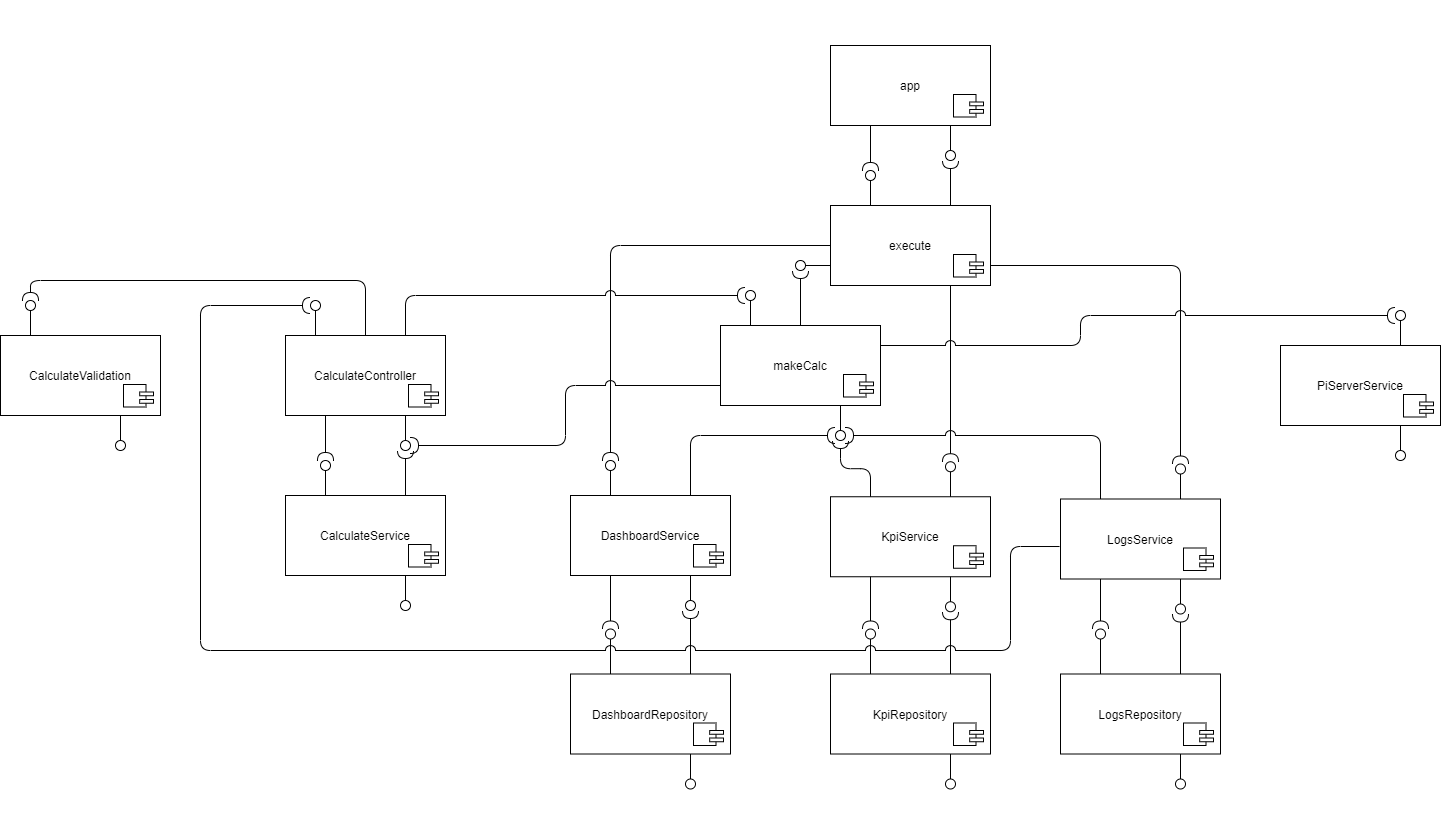
\includegraphics[width=14cm]{Metodologia/Figuras/kpiComponents.png}
	\caption{Diagrama de Componentes - Kpi-Executor}
	\label{fig:componentsKpi}
\end{figure}

Cada componente descrito no diagrama � composto por um arquivo independente em Python \cite{pyPage}, cada um com suas responsabilidades. 

\begin{itemize}
	\item \textbf{app:} Arquivo principal. Ele � o m�dulo invocado pelo orquestrador Kubernetes \cite{kubePage}. Respons�vel pela configura��o de logs de manuten��o e carregamento de vari�veis de ambiente do sistema, configurando a aplica��o para sua forma de execu��o local, em ambiente de valida��o ou produ��o;
	\item \textbf{execute:} Respons�vel por instanciar os objetos de banco de dados utilizados pelos pr�ximos componentes. Tamb�m invoca DashboardService para montar o objeto com os dados de cadastro para as etapas de c�lculos de KPIs;
	\item \textbf{makeCalc:} Opera o fluxo principal ta aplica��o. Percorre o objeto de dados de cadastro fornecido pelo componente \textit{execute} e solicitando, a cada itera��o, ao \textit{PiServerService} dados de processo cadastrados no PIMS, malha a malha;
	\item \textbf{DashboardService:} Possui regras de neg�cio relacionadas ao banco \textit{omo-db}. Formata os dados lidos e para inser��o neste banco. Tamb�m possui os m�todos para instanciar os objetos de banco de dados e para solicitar escrita no banco de dados;
	\item \textbf{DashboardRepository:} Possui os m�todos correspondentes �s queries de inser��o e consulta de dados em banco. Tem rela��o de heran�a \cite{engSw} com a classe \textit{Repository} (se��o \ref{sec:objDb});
	\item \textbf{PiServerService:} Contempla regras de neg�cio relacionadas � consulta de dados no PIMS. Formata e realiza requisi��es \textit{Http} para o m�dulo externo \textit{Pi-Connector} (figura \ref{fig:arqLoop}). Tamb�m possui rotinas para tratamento das respostas com os dados do PIMS;
	\item \textbf{KpiService:} Contempla as regras para formata��o de dados calculados para inser��o no banco \textit{omokpi};
	\item \textbf{LogsService:} Possui m�todos para conex�o com o banco de dados de logs de controle;
	\item \textbf{LogsRepository:} Possui m�todos relacionados a inser��o e leitura em dos logs em banco de dados. Tem rela��o de heran�a com a classe \textit{Repository} (se��o \ref{sec:objDb});
	\item \textbf{CalculateController:} Componente chave para o funcionamento da aplica��o. Contempla o fluxo descrito pelo levantamento de requisitos na figura \ref{fig:fluxoKpi}. Tamb�m invoca os m�dulos \textit{KpiService} e \textit{DashboardService} para registro de dados calculados e \textit{LogsService} para persist�ncia dos logs de controle;
	\item \textbf{CalculateService:} Possui os m�todos para a realiza��o dos c�lculos dos �ndices de performance. � invocado pelo \textit{calculateController};
	\item \textbf{CalculateValidation:} Possui m�todos auxiliares para a valida��o do fluxo de c�lculos. � invocado pelo \textit{CalulateController};
	
\end{itemize}

\paragraph{�ndices de Performance - KPIs}

\todo[inline]{Explicar os c�lculos realizados e citar a se��o (ainda n�o constru�da) da revis�o bibliogr�fica sobre os �ndices de performance.}

\paragraph{Registro de Logs de C�lculo}

\todo[inline]{Adicionar aqui o processo de estrutura��o dos logs de c�lculo em banco de dados. Associar esse processo ao fluxo da se��o de levantamento de requisitos.}


\subsubsection{Testes e Implanta��o}
\todo[inline]{Explicar etapas de teste com dados de cliente e valida��o de fluxo e resultados de c�lculos dos �ndices de performance}
\clearpage
%\chapter{Resultados}

Para a execu��o do projeto, algumas etapas de desenvolvimento tiveram de ser seguidas: familiariza��o com o sistema, estudo dos m�dulos envolvidos, leitura dos requisitos, elabora��o de documento descrevendo todo o processo de implementa��o e relacionamento com os diversos m�dulos, implementa��o e testes.

\section{Atividades do Projeto}
\markright{\thesection ~~~ Metodologia}
\label{metodo3}

\section {Requisitos do Sistema}
\markright{\thesection ~~~ Requisitos}
\label{req}






\begin{figure}[htbp]
\centering
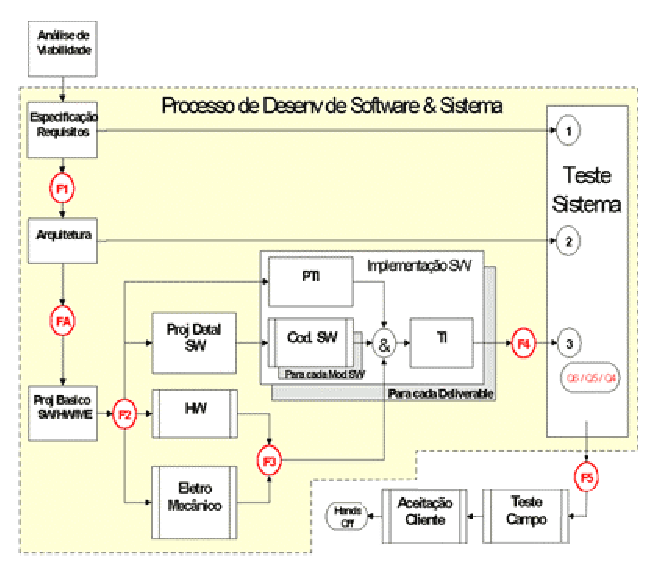
\includegraphics[scale=1.2]{Resultados/Figuras/ciclodesenvolvimento.eps}
\caption{Ciclo de desenvolvimento de um projeto}
\label{CicloDesenvolvimento}
\end{figure}

Para referenciar a Figura \ref{CicloDesenvolvimento}, veja arquivo .tex.



Aqui come�a uma sub-se��o.


\section{Desenvolvimeto e Implementa��o}

Aqui come�a outra se��o.

Para inserir a tabela abaixo, veja arquivo .tex.

\begin{table}
\centering
\begin{tabular}{|l|l|}\hline
		1.Uso do servi�o & Para o assinante rastrear uma chamada, ele dever� tirar\\ 
										 & o telefone do gancho, esperar pelo tom de discagem e ent�o \\
										 & discar o c�digo de acesso ao servi�o. \\ \hline
		2.Processamento  & Caso o assinante tenha acesso ao servi�o SRUC, ele dever�  \\			
		  do servi�o 		 & ouvir um an�ncio, ao discar o c�digo de acesso, explicando \\
									   & que o servi�o SRUC foi acessado. Dessa forma, se os dados \\
									   & a serem rastreados forem suficientes, o sistema dever� \\
									   & fornecer uma mensagem de confirma��o de \\
									   & servi�o realizado \\ \hline
		3. Ativa��o da   		& A ativa��o do servi�o somente ser� v�lida \\
			 �ltima chamada   & para a �ltima chamada recebida. \\ 
			 recebida				 	& \\ \hline
		4. Mais de uma   		& Se o assinante tentar ativar o servi�o para a mesma chamada \\
			 ativa��o para 	 	& ele dever� ouvir novamente o an�ncio de servi�o realizado, mas \\
			 a mesma chamada	& n�o ir� gravar os dados novamente \\ \hline
		5. N�mero privado 	& O sistema dever� mostrar o n�mero do assinante chamador \\
			 do assinante A  	& mesmo que este n�o possa ser mostrado. \\ \hline
		6. Chamadas  				& Para que o servi�o possa valer para chamadas intercentrais \\
			 intercentrais		& a central dever� utilizar a sinaliza��o SS7, e o n�mero do \\
												& assinante A ser� obtido pela mensagem IAM. \\ \hline
		7. Informa��es de 	& Um \textit{trace} do servi�o dever� possuir os seguintes itens:\\
			 um registro			& N�mero do assinante A \\
												& Hora da chamada recebida\\
												& Data da chamada recebida\\
												& N�mero do assinante B\\
												& Hora da solicita��o do servi�o\\
												& Data da solicita��o do servi�o\\
												& Dados sobre rota para chamadas intercentrais \\ \hline
		8. Tratamento para 	& Se um assinante discar o c�digo de acesso ao \\
		   assinante sem 		& servi�o, a central dever� fornecer tratamento padr�o \\
			 servi�o					& de acesso negado. \\ \hline
		9. Tipos de 				& A central deve permitir que o assinante com o servi�o \\
		   telefones				& possua tanto DTMF quando Dial Pulse \\ \hline
		10. Comandos do 		& O sistema supervis�rio conectado � central dever� \\
		    sistema 				& disponibilizar um  comando para que o operador possa  \\
		    supervis�rio		& descarregar o arquivo com os \textit{traces} das chamadas \\
		    								& para os diversos assinantes de uma central. \\
												& Um comando para visualizar os \textit{traces} tamb�m ser� necess�rio. \\ \hline
		\end{tabular}
	\caption{Requisitos do Servi�o SRUC}
	\label{tab:RequisitosDoServi�oSRUC}
\end{table}

Aqui voc� referencia a tabela: a Tabela \ref{tab:RequisitosDoServi�oSRUC} explicita os pontos mais relevantes na implementa��o do SRUC.

\section{Testes}

\section{Resumo do Cap�tulo}
\markright{\thesection ~~~ Metodologia}
\label{metodo4}
Esse cap�tulo pode ser dividido em duas partes $	f=ma $ blaba \cite{bel/00}
 
\begin{gather}
	f=ma\\
	x=2\\
\end{gather}

\begin{align}
	f=ma\\
	x=2\\
\end{align}

\begin{eqnarray}
	f=ma\\
	x=2\nonumber\\
\end{eqnarray}


\clearpage
%\chapter{Conclus�es}

\section{Considera��es Finais}

Aqui vai o texto da conclus�o.

\section{Propostas de Continuidade}


\clearpage


\addcontentsline{toc}{chapter}{Refer�ncias Bibliogr�ficas}
\bibliographystyle{plain}
\begin{small}
%\bibliography{telefonia}%,library}
\bibliography{references}
%% Monografia para Projeto de Fim de Curso - Felipe T. C. Ribeiro
%-----------------------------------------------------------


%---------------Inicializa��o de pacotes--------------------

\documentclass[12pt,a4paper,notitlepage,twoside]{book}
\usepackage{times}

\usepackage{graphicx}
\usepackage[latin1]{inputenc}
\usepackage[brazil]{babel}
\usepackage[T1]{fontenc}
\usepackage{amsmath}
\usepackage{amsthm,amsfonts}
\usepackage{color}
%\usepackage{hyperref}
\usepackage{abntex2abrev}


\usepackage[a4paper,top=30mm,bottom=30mm,inner=30mm,outer=25mm,headheight=7mm,headsep=6mm,footskip=7mm]{geometry}
%\usepackage{epsfig}
%\usepackage{latexsym}
%\usepackage{float}
%\usepackage{quotes}
%\pagestyle {plain}

\makeindex

\def\baselinestretch{1.0}

%---------------In�cio do documento-------------------------

\begin{document}

%\begin{titlepage}
\begin{center}
{\large Universidade Federal de Minas Gerais\\
Escola de Engenharia \\
Curso de Gradua��o em Engenharia de Controle e Automa��o\\}

\vspace{6cm}
{\bf\Large Aplica��o para c�lculo de indicadores de performance de malhas de controle de processos industriais\vspace{0.2cm}

%Segunda Linha do T�tulo, se Houver}
%\vspace{4cm}

%\hspace{0.3\textwidth} \parbox{0.65\textwidth}
{\large Felipe T. C. Ribeiro}
\vspace{2cm}  
   
\vspace{2cm}          
%\hspace{0.3\textwidth} 
{\large Orientador: Prof. Frederico Gualberto Ferreira Coelho.}\\
{\large Supervisor: Eng. Bernardo William Cafiero Viana}

\vfill
%\hspace{0.3\textwidth} 
{\large Belo Horizonte, Dezembro de 2020 }
\end{center}

\end{titlepage}

\newpage
\clearpage
\thispagestyle{empty}


\begin{titlepage}

\centering
\textbf{Monografia}\\
\vspace{2cm}
\centering
\textbf{Aplica��o para c�lculo de indicadores de performance de malhas de controle de processos industriais}\\
\vspace{5cm} 

\parbox{1.0\textwidth} 
{\large 
Monografia submetida � banca examinadora
designada pelo Colegiado Did�tico do Curso de
Gradua��o em Engenharia de Controle e
Automa��o da Universidade Federal de Minas
Gerais, como parte dos requisitos para aprova��o na
disciplina Projeto Final de Curso II.}

\vspace{7cm} 
\centering
Belo Horizonte, Julho de 2014

\end{titlepage}

\clearpage
\thispagestyle{empty}
\cleardoublepage

\pagenumbering{roman}
%\addcontentsline{toc}{chapter}{Resumo}

\begin{center}
\huge{{\bf Resumo}}
\vspace{2cm}
\end{center}
 
O presente trabalho apresenta o processo de desenvolvimento de uma aplica��o para c�lculo de �ndices de performance de malhas de controle, implantada em conjunto a um sistema CPM, sigla do ingl�s para \textit{Controller Performance Monitoring}, que recebe o nome de LOOP, desenvolvido pela empresa \textit{IHM Stefanini}. O sistema em quest�o � utilizado por um conjunto de diferentes clientes da ind�stria nacional como ferramenta para acompanhamento e metrifica��o dos estados de suas malhas de controle. Para tais avalia��es � comum a utiliza��o de �ndices de performance, que traduzem a n�meros, o desempenho de um sistema de controle. Nesse ponto entra a aplica��o alvo desse projeto, que recebe o nome de Kpi-Executor. O Kpi-Executor foi constru�do para a realiza��o dos c�lculos dos �ndices de performance, do ingl�s \textit{Key Performance Indicators}, abreviado por KPIs, que s�o parte essencial do sistema LOOP. � desejado que esta aplica��o se integre sem problemas ao sistema existente, em substitui��o a uma anterior com fun��o semelhante, tendo sua execu��o realizada a cada hora, gerando assim os valores desses �ndices utilizados. Nessa monografia ser�o detalhados o processo de desenvolvimento desse software, al�m da concep��o te�rica dos �ndices de performance os utilizados pelo sistema: Tempo em modo normal, Tempo sem satura��o, Erro m�dio aceit�vel e Nota global. Como resultados s�o apresentados documenta��o de regras de neg�cio gerada, a estrutura de logs para melhoria na etapa de manuten��o e evolu��o do software, al�m da estabiliza��o e repetibilidade obtidas pelo Kpi-Executor. 
 
%\begin{sloppypar}
%Este novo par�grafo serve para mostrar que ao pular uma ou mais linhas no texto do arquivo .tex, o \TeX\ entende que voc� est� iniciando outro par�grafo. O comando sloppypar for�a o texto a n�o ultrapassar as margens. S� deve ser usado se este problema ocorrer.
%\end{sloppypar}

 
\clearpage
\thispagestyle{empty}
\cleardoublepage


%\addcontentsline{toc}{chapter}{Agradecimentos}

\begin{center}
\huge{{\bf Agradecimentos}}
\vspace{4cm}
\end{center}

\begin{center}
	\begin{quotation}
		{\bf "Pra que amanh\~{a} n\~{a}o seja s\'{o} um ontem com um novo nome", Leandro}
	\end{quotation}
\end{center}



A Deus pela coragem e for\c{c}a concedida. \`{A} minha m\~{a}e, S\^{o}nia, pelo exemplo de for\c{c}a, resili\^{e}ncia e por todo apoio e ensinamento sobre jornadas. Ao meu pai por sua import\^{a}ncia no meu amadurecimento. \`{A}s minhas amigas e colegas de curso Lud, Manu e Pena que sabem exatamente o porque de estarem aqui. \`{A} expans\~{a}o da minha fam\'{i}lia nas pessoas de Gutenberg, Lidiane, Let\'{i}cia e av\'{o}s. A todos os amigos de caminhada. Por fim, n\~{a}o menos importante, minha esposa, Larissa.


\begin{center}
	\begin{quotation}
		{\bf M\~{a}e! A favela venceu!}
	\end{quotation}
\end{center}

 
\clearpage
\thispagestyle{empty}
\cleardoublepage
%\setcounter{tocdepth}{3}
\setcounter{secnumdepth}{3}
\tableofcontents
%\markboth{Conte�do}{Conte�do}

\clearpage
%\thispagestyle{empty}
%\cleardoublepage

% Normalmente, este arquivo s� cont�m isto.
%\listoffigures
\addcontentsline{toc}{chapter}{Lista de Figuras}
%\markboth{Lista de Figuras}{Lista de Figuras}

\clearpage
%\thispagestyle{empty}
%\cleardoublepage

% Normalmente, este arquivo s� cont�m isto.
%\listoftables
\addcontentsline{toc}{chapter}{Lista de Tabelas}
%\markboth{Lista de Tabelas}{Lista de Tabelas}

\clearpage
\thispagestyle{empty}
\cleardoublepage

% Normalmente, este arquivo s� cont�m isto.

\pagenumbering{arabic}
\setcounter{page}{1}
\chapter{Introdu��o}
\markright{\thechapter ~~~ Introdu��o}
%\label{intro}

%Se preferir, voc� pode apresentar este Cap�tulo antes da primeira Se��o, destacando os principais pontos que s�o abordados. %\cite{Raffo2008}

\section{Motiva��o e Justificativa}
%\markright{\thesection ~~~ Motiva��o}
%\label{motiva}

� incontest�vel a incessante busca do setor industrial pelo aumento do desempenho de suas unidades operacionais. Para que as empresas envolvidas nesse ramo possam se manter de forma significativa no mercado, � necess�ria a constante reavalia��o de seus processos, bem como de seus custos com energia, perdas e reprocessamento de material. Independentemente do setor de atua��o da ind�stria a ser avaliada, tais fatores possuem extrema import�ncia, devendo ser monitoradas, controladas e projetadas.

Para elucidar, tomemos como exemplo um processo de beneficiamento min�rio de ferro. Pode-se dividi-lo em: Britagem, peneiramento, moagem, classifica��o, concentra��o, espessamento e filtragem. Cada uma dessas etapas � composta por vari�veis a serem controladas de forma individual, como n�veis de tanque, temperatura e densidade de misturas, velocidades de motores, posi��es de v�lvulas, etc. Para estabelecer o comportamento desejado para tais processos, se faz necess�ria a aplica��o de estrat�gias de controle regulat�rio, avan�ado ou de outras naturezas. O conjunto composto por vari�vel a ser controlada e estrat�gia de controle utilizada � chamado de \textit{malha de controle}.

Implementado um sistema de controle, obt�m-se ent�o um processo minimamente adequado aos par�metros configurados para o contexto operacional escolhido. Entretanto, n�o menos importante que essa adequa��o t�cnica individual estabelecida por esse sistema, s�o os resultados e efeitos colaterais gerados naquela linha do processo,  bem como a avalia��o do conjunto em situa��es n�o previstas nas estrat�gias de controle. Dessa forma, o acompanhamento e metrifica��o do comportamento de sistemas de controle industriais ganha notabilidade dentro do setor industrial.


Para este monitoramento s�o utilizados softwares baseadis em CPM (\textit{Controller Performance Monitoring}). Eles possuem ferramental para an�lise temporal das malhas envolvidas,  avalia��o de par�metros de controladores, modelagem de processos e medi��o de KPIs (\textit{Key Performance Indicators}). Buscando este espa�o de mercado, a empresa IHM Stefanini desenvolveu o software LOOP, que se enquadra no tipo citado.

Nos �ltimos meses o time de desenvolvimento da empresa iniciou, juntamente ao time de analistas de controle que utilizam o sistema, um processo de identifica��o de pontos de melhoria do software LOOP, envolvendo quesitos de interface, regras de neg�cio, distribui��o de responsabilidades entre os m�dulos do sistema, arquitetura, integra��o de c�digo e documenta��o. Dentre os pontos n�o satisfat�rios listados pela equipe, o m�dulo respons�vel pelo c�lculo de KPIs foi apontado como cr�tico, sendo o primeiro a passar por mudan�as significativa. O projeto descrito por esta monografia aborda o processo de reconstru��o desse m�dulo.


\section{Objetivos do Projeto}
%\markright{\thesection ~~~ Objetivos}
%label{objetivos}

O objetivo do projeto � a constru��o de um m�dulo para c�lculo de �ndices de performance, utilizando-se de conhecimentos de Engenharia de software e desenvolvimento de sistemas. Como requisitos para aceita��o, o m�dulo deve possuir as seguintes caracter�sticas:
\begin{itemize}
	\item \textbf{Execu��o c�clica:} O c�lculo dos �ndices de performance � baseado em janelas de dados de uma hora. Dessa forma, ele deve possuir execu��o c�clica com um intervalos semelhantes;
	\item \textbf{Adequa��o � estrutura do sistema:} O m�dulo ser� utilizado para compor um sistema da empresa parceira, Ihm Stefanini, que j� possui outros m�dulos existentes. Assim � necess�rio que sejam respeitadas limita��es e conceitos do sistema como um todo;
	\item \textbf{Registro de falhas:} � necess�rio que o m�dulo apresente registros de falhas de cada uma das execu��es, n�o somente listando, mas tamb�m identificando quais tipos;
\end{itemize}




\section{Local de Realiza��o}
\label{sec:ihm}
%\markright{\thesection ~~~ A Empresa}
%\label{empresa}
O projeto de fim de curso foi desenvolvido em parceria com a empresa IHM Stefanini, no setor de Discovery da mesma, respons�vel pelo desenvolvimento, evolu��o e manuten��o da arquitetura e c�digo fonte dos sistemas ali desenvolvidos. O posto de trabalho variou entre as depend�ncias da empresa, e regime de \textit{home office}, conforme necess�rio.

A empresa realiza projetos e desenvolvimentos de Automa��o, El�trica, Montagem, bem como servi�os de otimiza��o de malhas, projetos de controle avan�ado e gest�o. Atua em diversas �reas da ind�stria, como Minera��o, Siderurgia \& Metais, Papel \& Celulose, e �leo \& G�s. 

A IHM Stefanini foi criada em 1994 inicialmente com o nome de IHM como uma integradora de sistemas, instrumenta��o, el�trica e TI Industrial. Com sua expans�o, passa a fazer parte do grupo Stefanini em 2015. A partir da� funda o departamento de inova��o e come�a a atuar na busca por tecnologias disruptivas e elabora��o de produtos digitais.

Atualmente a IHM Stefanini � dividida nos seguintes setores t�cnicos:
\begin{itemize}
	\item Departamento de TA;
	\item Departamento de TI Industrial;
	\item Departamento Intelig�ncia Industrial;
	\item Departamento de Discovery;
	\item Departamento de El�trica;
\end{itemize}

Este projeto foi desenvolvido no departamento de Discovery que tem como prop�sito a descoberta sistem�tica e estrutura��o de ofertas de alto valor agregado para a empresa. Subdividido em:
\begin{itemize}
	
	\item Produtos: Forma��o de produtos que resolvam problemas reais de clientes finais;
	\item Coder: Time respons�vel pelos softwares do setor. Estrutura, desenvolve e mant�m c�digos-fonte e infraestruturas das demandas do setor.
	
\end{itemize}



\section{Estrutura da Monografia}
%\markright{\thesection ~~~ Organiza��o do Trabalho}
\label{estruturaMono}

O trabalho est� estruturado em quatro cap�tulos, sendo o Cap�tulo 1 o conjunto contextualiza��o, relev�ncia e principais objetivos do projeto como um todo. O Cap�tulo 2 contempla apresenta��o e revis�o de conceitos b�sicos importantes para melhor entendimento do projeto. J� o Cap�tulo 3 traz informa��es sobre os recursos necess�rios, metodologia de desenvolvimento e implementa��o do projeto. No Cap�tulo 4, a apresenta��o e discuss�o de dados, bem como sugest�es e dificuldades a serem encontradas no projeto. Por fim, no Cap�tulo 5, s�o apresentadas as conclus�es obtidas no ap�s a elabora��o do projeto, e considera��es sobre poss�veis continuidades.

%\chapter{Descri��o do Processo}

Se desejar, uma vis�o geral do Cap�tulo pode ser colocada antes da primeira Se��o. Este � o cap�tulo de descri��o do processo e formula��o do problema. Tendo em vista que se trata de uma monografia de engenharia de controle e automa��o, em muitos casos, � fundamental a apresenta��o dos sensores e atuadores do processo.


\section{Processo de Fazer Alguma Coisa}
\markright{\thesection ~~~ Hist�rico}
\label{hist}

...


\section{Instrumenta��o do Processo}
\markright{\thesection ~~~ O Telefone}
\label{telefone}



Continua ...


\section{Resumo do Cap�tulo}

N�o termine de forma abrupta.



\clearpage

%\chapter{Materiais e M�todos}
\markright{\thechapter ~~~ Metodologia}
Neste cap�tulo s�o descritos os recursos de hardware e software necess�rios para o desenvolvimento deste projeto. S�o listados IDE utilizada para desenvolvimento, arquitetura existente a consumir dados da aplica��o e escolha de algoritmos de c�lculo de KPIs. Tamb�m s�o apresentados os processos de desenvolvimento de software utilizados e funcionamento da equipe dentro da qual foi o projeto foi constru�do.

\section{Descri��o de Componentes}

Esta se��o apresenta a arquitetura existente que receber� a aplica��o desenvolvida, o Kpi-Executor, bem como os recursos de hardware e software utilizados no seu desenvolvimento.

\subsection{Software}

\subsubsection{IDE, Linguagem e Banco de Dados}

Para o desenvolvimento da aplica��o foi escolhida a linguagem \textit{Python} \cite{pyPage}, em sua vers�o $3.8$, devido a seu car�ter de alto n�vel e sua grande gama de bibliotecas dispon�veis. Para a codifica��o foi escolhida a IDE \textit{Visual Studio Code} \cite{vscodePage}, devido � sua multiplicidade de extens�es e tamb�m por j� ser amplamente utilizada pela comunidade de desenvolvedores de software.

Ambas, linguagem e IDE, tem caracter�stica \textit{opensource}, sendo ativamente utilizadas e exploradas dia a dia por sua ampla comunidade, al�m de terem seus m�dulos e extens�es gratuitos.

Quanto ao armazenamento dos dados, foi utilizada uma estrutura relacional de banco de dados, considerando sua praticidade, bem como a estrutura existente descrita nas pr�ximas se��es. Foi utilizada uma inst�ncia de um banco de dados \textit{PostgresSQL} \cite{postgresPage} , uma ferramenta gratuita para a persist�ncia dos dados gerados pela aplica��o.

\subsubsection{Orquestradores e Containers}

Como a aplica��o desenvolvida foi acoplada a um sistema existente, foi necess�rio que ela respeitasse o conjunto anteriormente elaborado, bem como se adequasse � arquitetura em nuvem \cite{cloudComp} j� em funcionamento. Para tal, essa aplica��o deveria possuir certo encapsulamento.

Uma forma amplamente utilizada para o encapsulamento e execu��o de aplica��es de grande porte � o formato de \textit{containers}. � uma abordagem de desenvolvimento de software onde um servi�o ou aplicativo � empacotado com suas depend�ncias e configura��es \cite{containerIntr}. Dessa forma, s�o facilitados os processos de Testes de unidade e integra��o \cite{engSw}, bem como etapas de evolu��o \cite{engSw} e versionamento daquele conjunto. Para o processo de constru��o de \textit{container} do m�dulo \textit{Kpi-Executor} foi utilizada a plataforma \textit{Docker} \cite{dockerPage}, gerando uma imagem de um SO (Sistema Operacional) Linux contendo as depend�ncias e instala��es necess�rias para a execu��o do \textit{Kpi-Executor}.

Uma vez empacotada a aplica��o, � necess�rio utilizar uma ferramenta para operar esse pacote, o executando sempre que necess�rio. Esta utilidade � chamada de \textit{orquestrador}. A ferramenta deste tipo utilizada foi o \textit{Kubernetes} \cite{kubePage}. Este tipo de ferramenta possibilita a automa��o de opera��es \textit{containers}, como implanta��es ou atualiza��es das aplica��es, o gerenciamento de servi�os de forma declarativa garantindo a repetibilidade do sistema, a separa��o de \textit{containers} em diferentes \textit{hosts}, bem como a verifica��o de integridade e autorrecupera��o das aplica��es \cite{whatKube}.


\subsection{Estrutura Existente}

A aplica��o constru�da funcionar� como um m�dulo de um sistema de CPM existente chamado LOOP. Ele � composto por um conjunto de m�dulos, cada um com sua responsabilidade bem definida. A figura \ref{fig:arqLoop} traz o esquema arquitetural do sistema, bem como o relacionamento entre os m�dulos.

\begin{figure}[!htbp]
	\centering		
	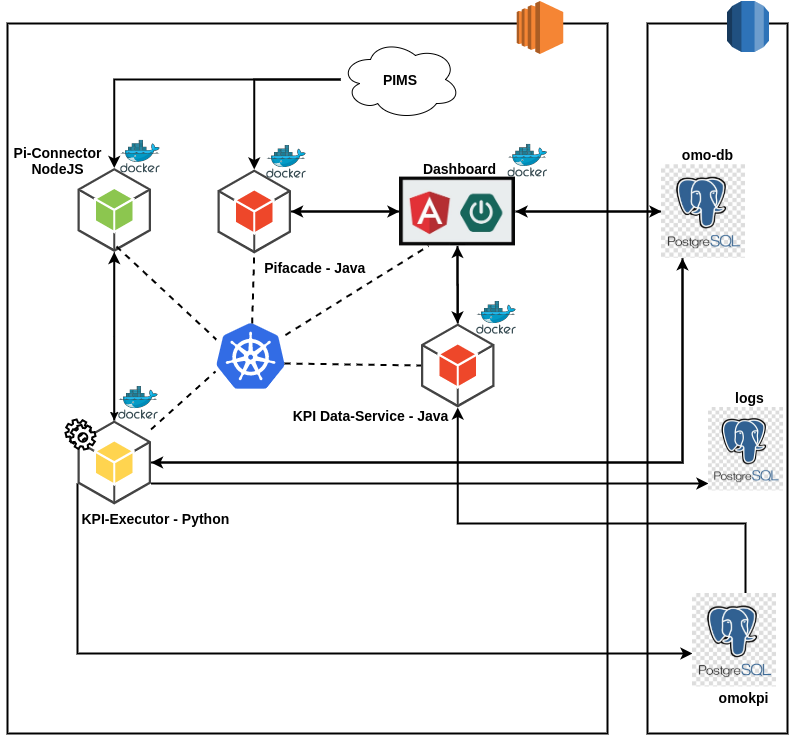
\includegraphics[width=10cm]{Metodologia/Figuras/arquitetura-omo.png}
	\caption{Arquitetura Loop}
	\label{fig:arqLoop}
\end{figure}

Neste esquema s�o identificadas as linguagens e tecnologias de cada m�dulo. S�o eles:

\begin{itemize}
	\item \textbf{Dashboard:} Aplica��o web acess�vel ao usu�rio do sistema CPM LOOP composta por um \textit{backend} em \textit{Spring Boot} \cite{springBootPage} e \textit{frontend} em \textit{AngularJS} \cite{angularJSPage};
	\item \textbf{Bancos de Dados:} S�o tr�s inst�ncias de banco de dados do sistema. A nomeada como \textit{omo-db} carrega as informa��es de cadastro e configura��o das entidades do LOOP. A nomeada \textit{omokpi} armazena os dados calculados pelo Kpi-Executor, enquanto a \textit{logs} registra os logs de funcionamento da aplica��o de c�lculos. Todas as inst�ncias s�o do tipo PostgreSQL \cite{postgresPage};
	\item \textbf{Data-Service:} M�dulo do tipo API constru�do em \textit{Spring Boot} \cite{springBootPage} respons�vel por prover dados registrados no banco \textit{omokpi} � aplica��o web \textit{Dashboard}. Formata pesquisa e retorna dados sob demanda;
	\item \textbf{PIMS:} Um sistema PIMS da \textit{OsiSoft} chamado \textit{PI System} \cite{piPage}. Nele s�o armazenados os dados de processo dos clientes que utilizam o sistema LOOP. Estes dados s�o utilizados na realiza��o dos c�lculos (Kpi-Executor);
	\item \textbf{Pi-Facade:} M�dulo do tipo API constru�do em \textit{Spring Boot} \cite{springBootPage} respons�vel por prover dados registrados e cadastrar novas informa��es no PIMS sob demanda da aplica��o web \textit{Dashboard};
	\item \textbf{Pi-Connector:} M�dulo do tipo API constru�do em \textit{NodeJS} \cite{nodejsPage} respons�vel pelo fornecimento de dados registrados no PIMS � aplica��o de c�lculos (Kpi-Executor);
	\item \textbf{Kpi-Executor:} M�dulo desenvolvido descrito por esta monografia. Constru�do em \textit{Python 3.8} \cite{pyPage} e respons�vel por calcular os �ndices de performance (KPIs) do sistema LOOP. Opera de forma c�clica, realizando seus c�lculos a cada hora.
	
\end{itemize}


\newpage
\subsection{Hardware}
Para realiza��o do desenvolvimento do Kpi-Executor, foi necess�rio um notebook com 16Gb de mem�ria e processador intel i7. Tamb�m foi necess�rio um ambiente de Testes e valida��o semelhante ao de produ��o. S�o m�quinas hospedadas na \textit{Amazon Web Services} \cite{awsHome}.



\section{Metodologia}
%\markright{\thesection ~~~ Metodologia}

Para a constru��o dessa aplica��o foi utilizado o um processo de desenvolvimento de software composto por caracter�sticas de um cascata e um incremental \cite{engSw}. Como o projeto foi entendido como uma demanda associada ao fluxo de trabalho da equipe de Coder, descrita na se��o \ref{sec:ihm}, ele estava submetido a um fluxo de \textit{Kanban}, o que aponta para o quesito de entrega incremental quando associado ao sistema LOOP como um todo. Entretanto, como se tratava de uma tarefa n�o pequena, foram necess�rias etapas que coincidem com o processo cascata.
Neste cap�tulo ser�o listadas as etapas de projeto, desenvolvimento e testes do Kpi-Executor, bem como as escolhas relacionadas aos c�lculos por ele realizados.

\subsection{Processo de Desenvolvimento}

O processo de desenvolvimento da aplica��o iniciou-se com um escopo relativamente simples. Ela deveria realizar de forma c�clica um conjunto de c�lculos de �ndices de performance que s�o utilizados pelo sistema CPM LOOP, registr�-los em um banco de dados existente, com estrutura tamb�m definida, e possibilitar um rastreio de falhas no fluxo de c�lculos, identificando o qual tipo de erro, e em que momento este acontecera. Tendo essas informa��es, ainda foi eram necess�rias mais defini��es de casos espec�ficos n�o mapeados pela descri��o inicial. 

\subsubsection{Levantamento do Requisitos}

Considerando a necessidade de um mapeamento detalhado dos casos de c�lculo, foi realizado um processo de entrevista com o PO (\textit{Product Owner}) do sistema LOOP, a fim de elucidar o fluxo de c�lculo em seu estado ideal, poss�veis tratativas em casos n�o usuais e demais requisitos funcionais e n�o-funcionais. Deste levantamento, foi elaborado o diagrama de sequ�ncia (\ref{sec:modSeq}) tratando o fluxo a ser executado pelo Kpi-Executor, exibido na figura (\ref{fig:fluxoKpi}).

 \begin{figure}[!htbp]
 	\centering		
 	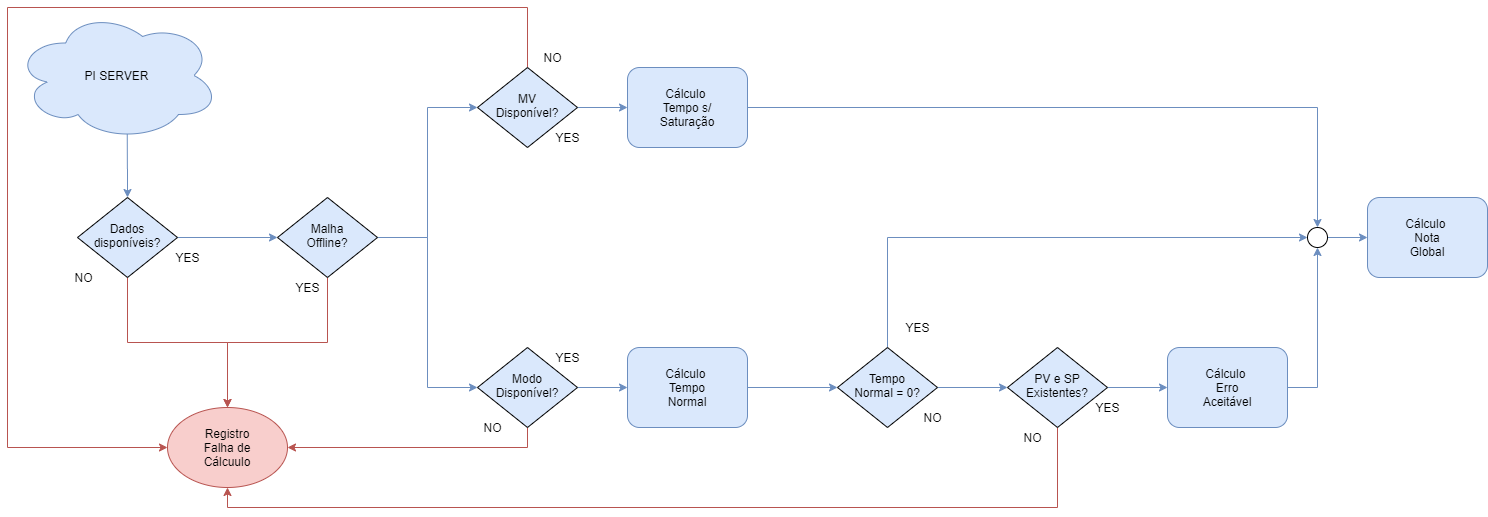
\includegraphics[width=14cm]{Metodologia/Figuras/fluxoKpiExecutor.png}
 	\caption{Diagrama de Sequ�ncia - Kpi-Executor}
 	\label{fig:fluxoKpi}
 \end{figure}
 
Ap�s constru��o deste diagrama de alto n�vel, foi realizada o nova reuni�o o validando como fluxo correto de c�lculos, incluindo as tratativas de casos espec�ficos. Assim p�de-se caminhar para a pr�xima etapa do processo.

\subsubsection{Projeto da Aplica��o}

Tendo requisitos funcionais e n�o-funcionais especificados, foi poss�vel ent�o o in�cio do projeto da aplica��o. Inicia-se pela defini��o arquitetural do m�dulo Kpi-Executor. Foi escolhida uma arquitetura em camadas (se��o \ref{sec:arqCamadas}) devido � familiaridade da equipe com o tipo de constru��o e a seu car�ter de atua��o sob demanda e persist�ncia em banco de dados. 

Para persist�ncia dos dados em banco, foi escolhida a tecnologia SQLAlchemy \cite{alchemyPage}, amplamente utilizada para acesso via Python a bancos de dados relacionais. Ela possibilita uma abordagem de orienta��o a objetos (se��o \ref{sec:seqOO}) em sua utiliza��o.

\subsubsection{Desenvolvimento da Aplica��o}

\paragraph {Classes auxiliares}
\label{sec:objDb}
Considerando a estrutura do sistema da empresa parceira (Loop) no momento do desenvolvimento do m�dulo tratado por essa monografia, era tido como de suma import�ncia a possibilidade de utiliza��o de diferentes bancos de dados relacionais, como Microfost SQL Server \cite{sqlServerHome} e PostgresSQL \cite{postgresPage}. Assim, foi necess�ria a utiliza��o da uma \textit{ORM} (Object Relacional Mapper) \cite{ORM} \textit{SQLAlchemy} \cite{alchemyPage}, possibilitando que o m�dulo em quest�o apresentasse caracter�sticas agn�sticas a banco de dados. Al�m da facilita��o no processo de substitui��o de bancos de dados, devido � objetifica��o das \textit{queries} adiciona seguran�a ao conjunto do sistema, impedindo tentativas de invas�o do tipo \textit{SQL Injection} \cite{SQLInjection}.

Uma vez levantados os pontos citados, foram utilizados os conceitos de orienta��o a objetos para o desenvolvimento (\ref{sec:seqOO}) para a elabora��o de duas classes que juntas tornariam o processo de constru��o das consultas e inser��es a banco de dados mais pr�ticas e robustas:

\begin{itemize}
	\item \textbf{Database:} Classe que contempla m�todos para conex�o e desconex�o com o banco de dados, bem como as informa��es de conex�o, como \textit{host}, nome do banco, usu�rio, senha e \textit{driver}. Seu uso consiste na representa��o de um banco de dados como um objeto. O \textit{SQLAlchemy} \cite{alchemyPage} faz gerenciamento autom�tico de m�ltiplas conex�es, possibilitando o instanciamento de diversos objetos dessa classe;
	\item \textbf{Repository:} Classe que contempla os m�todos b�sicos relacionados a consultas, inser��es, atualiza��es e dele��es. Seu uso consiste em t�-la como pai para cada nova classe com fun��es de acesso a dados. Possui um atributo do tipo \textit{Database} que aponta para o banco de dados a ser utilizado.
\end{itemize}

Uma vez elaboradas tais classes auxiliares, tem-se a etapa seguinte que contempla o conceito de divis�o de camadas (\ref{sec:arqCamadas}), novamente orienta��o a objetos (\ref{sec:seqOO}) e modelagem orientada a dados (\ref{sec:modSeq}).

\paragraph{Divis�o de Responsabilidades}

Considerando uma arquitetura de camadas, o Kpi-Executor foi modularizado dividindo as responsabilidades entre estes m�dulos. Foram separadas entre os componentes as tarefas de se consumir e escrever em diferentes bases de dados, operar o fluxo de c�lculos, registrar exce��es e falhas de c�lculo, etc. A figura \ref{fig:componentsKpi} traz o diagrama de componentes que descreve tal modulariza��o.

\begin{figure}[!htbp]
	\centering		
	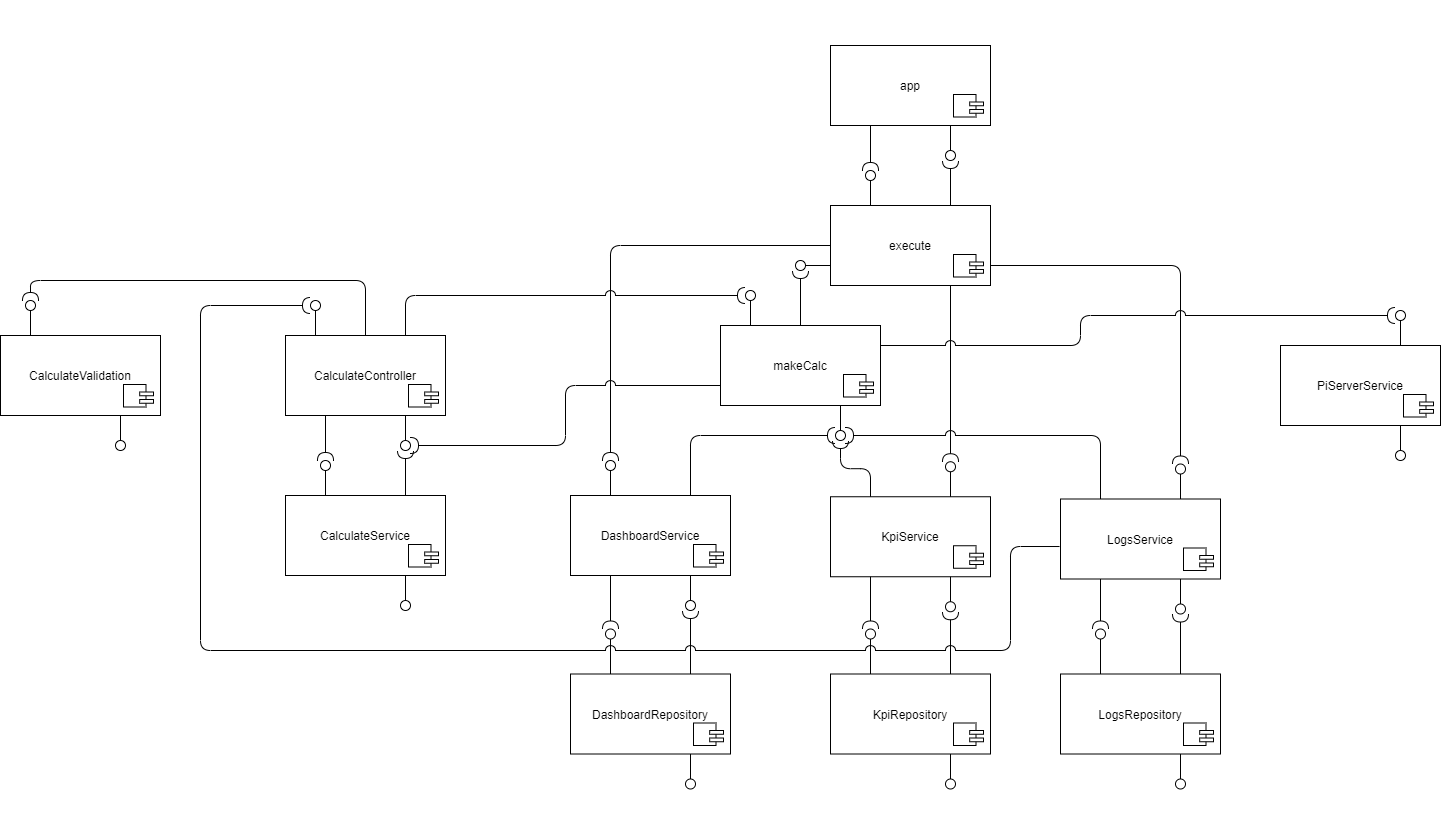
\includegraphics[width=14cm]{Metodologia/Figuras/kpiComponents.png}
	\caption{Diagrama de Componentes - Kpi-Executor}
	\label{fig:componentsKpi}
\end{figure}

Cada componente descrito no diagrama � composto por um arquivo independente em Python \cite{pyPage}, cada um com suas responsabilidades. 

\begin{itemize}
	\item \textbf{app:} Arquivo principal. Ele � o m�dulo invocado pelo orquestrador Kubernetes \cite{kubePage}. Respons�vel pela configura��o de logs de manuten��o e carregamento de vari�veis de ambiente do sistema, configurando a aplica��o para sua forma de execu��o local, em ambiente de valida��o ou produ��o;
	\item \textbf{execute:} Respons�vel por instanciar os objetos de banco de dados utilizados pelos pr�ximos componentes. Tamb�m invoca DashboardService para montar o objeto com os dados de cadastro para as etapas de c�lculos de KPIs;
	\item \textbf{makeCalc:} Opera o fluxo principal ta aplica��o. Percorre o objeto de dados de cadastro fornecido pelo componente \textit{execute} e solicitando, a cada itera��o, ao \textit{PiServerService} dados de processo cadastrados no PIMS, malha a malha;
	\item \textbf{DashboardService:} Possui regras de neg�cio relacionadas ao banco \textit{omo-db}. Formata os dados lidos e para inser��o neste banco. Tamb�m possui os m�todos para instanciar os objetos de banco de dados e para solicitar escrita no banco de dados;
	\item \textbf{DashboardRepository:} Possui os m�todos correspondentes �s queries de inser��o e consulta de dados em banco. Tem rela��o de heran�a \cite{engSw} com a classe \textit{Repository} (se��o \ref{sec:objDb});
	\item \textbf{PiServerService:} Contempla regras de neg�cio relacionadas � consulta de dados no PIMS. Formata e realiza requisi��es \textit{Http} para o m�dulo externo \textit{Pi-Connector} (figura \ref{fig:arqLoop}). Tamb�m possui rotinas para tratamento das respostas com os dados do PIMS;
	\item \textbf{KpiService:} Contempla as regras para formata��o de dados calculados para inser��o no banco \textit{omokpi};
	\item \textbf{LogsService:} Possui m�todos para conex�o com o banco de dados de logs de controle;
	\item \textbf{LogsRepository:} Possui m�todos relacionados a inser��o e leitura em dos logs em banco de dados. Tem rela��o de heran�a com a classe \textit{Repository} (se��o \ref{sec:objDb});
	\item \textbf{CalculateController:} Componente chave para o funcionamento da aplica��o. Contempla o fluxo descrito pelo levantamento de requisitos na figura \ref{fig:fluxoKpi}. Tamb�m invoca os m�dulos \textit{KpiService} e \textit{DashboardService} para registro de dados calculados e \textit{LogsService} para persist�ncia dos logs de controle;
	\item \textbf{CalculateService:} Possui os m�todos para a realiza��o dos c�lculos dos �ndices de performance. � invocado pelo \textit{calculateController};
	\item \textbf{CalculateValidation:} Possui m�todos auxiliares para a valida��o do fluxo de c�lculos. � invocado pelo \textit{CalulateController};
	
\end{itemize}

\paragraph{�ndices de Performance - KPIs}

\todo[inline]{Explicar os c�lculos realizados e citar a se��o (ainda n�o constru�da) da revis�o bibliogr�fica sobre os �ndices de performance.}

\paragraph{Registro de Logs de C�lculo}

\todo[inline]{Adicionar aqui o processo de estrutura��o dos logs de c�lculo em banco de dados. Associar esse processo ao fluxo da se��o de levantamento de requisitos.}


\subsubsection{Testes e Implanta��o}
\todo[inline]{Explicar etapas de teste com dados de cliente e valida��o de fluxo e resultados de c�lculos dos �ndices de performance}
\clearpage
%\chapter{Resultados}

Para a execu��o do projeto, algumas etapas de desenvolvimento tiveram de ser seguidas: familiariza��o com o sistema, estudo dos m�dulos envolvidos, leitura dos requisitos, elabora��o de documento descrevendo todo o processo de implementa��o e relacionamento com os diversos m�dulos, implementa��o e testes.

\section{Atividades do Projeto}
\markright{\thesection ~~~ Metodologia}
\label{metodo3}

\section {Requisitos do Sistema}
\markright{\thesection ~~~ Requisitos}
\label{req}






\begin{figure}[htbp]
\centering
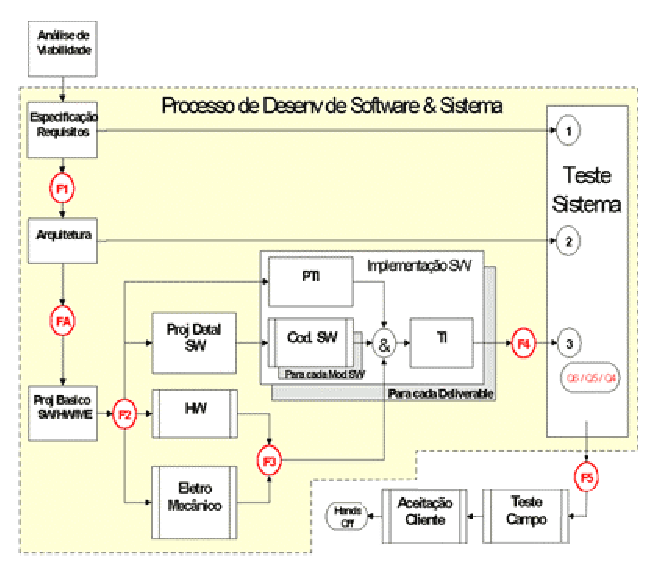
\includegraphics[scale=1.2]{Resultados/Figuras/ciclodesenvolvimento.eps}
\caption{Ciclo de desenvolvimento de um projeto}
\label{CicloDesenvolvimento}
\end{figure}

Para referenciar a Figura \ref{CicloDesenvolvimento}, veja arquivo .tex.



Aqui come�a uma sub-se��o.


\section{Desenvolvimeto e Implementa��o}

Aqui come�a outra se��o.

Para inserir a tabela abaixo, veja arquivo .tex.

\begin{table}
\centering
\begin{tabular}{|l|l|}\hline
		1.Uso do servi�o & Para o assinante rastrear uma chamada, ele dever� tirar\\ 
										 & o telefone do gancho, esperar pelo tom de discagem e ent�o \\
										 & discar o c�digo de acesso ao servi�o. \\ \hline
		2.Processamento  & Caso o assinante tenha acesso ao servi�o SRUC, ele dever�  \\			
		  do servi�o 		 & ouvir um an�ncio, ao discar o c�digo de acesso, explicando \\
									   & que o servi�o SRUC foi acessado. Dessa forma, se os dados \\
									   & a serem rastreados forem suficientes, o sistema dever� \\
									   & fornecer uma mensagem de confirma��o de \\
									   & servi�o realizado \\ \hline
		3. Ativa��o da   		& A ativa��o do servi�o somente ser� v�lida \\
			 �ltima chamada   & para a �ltima chamada recebida. \\ 
			 recebida				 	& \\ \hline
		4. Mais de uma   		& Se o assinante tentar ativar o servi�o para a mesma chamada \\
			 ativa��o para 	 	& ele dever� ouvir novamente o an�ncio de servi�o realizado, mas \\
			 a mesma chamada	& n�o ir� gravar os dados novamente \\ \hline
		5. N�mero privado 	& O sistema dever� mostrar o n�mero do assinante chamador \\
			 do assinante A  	& mesmo que este n�o possa ser mostrado. \\ \hline
		6. Chamadas  				& Para que o servi�o possa valer para chamadas intercentrais \\
			 intercentrais		& a central dever� utilizar a sinaliza��o SS7, e o n�mero do \\
												& assinante A ser� obtido pela mensagem IAM. \\ \hline
		7. Informa��es de 	& Um \textit{trace} do servi�o dever� possuir os seguintes itens:\\
			 um registro			& N�mero do assinante A \\
												& Hora da chamada recebida\\
												& Data da chamada recebida\\
												& N�mero do assinante B\\
												& Hora da solicita��o do servi�o\\
												& Data da solicita��o do servi�o\\
												& Dados sobre rota para chamadas intercentrais \\ \hline
		8. Tratamento para 	& Se um assinante discar o c�digo de acesso ao \\
		   assinante sem 		& servi�o, a central dever� fornecer tratamento padr�o \\
			 servi�o					& de acesso negado. \\ \hline
		9. Tipos de 				& A central deve permitir que o assinante com o servi�o \\
		   telefones				& possua tanto DTMF quando Dial Pulse \\ \hline
		10. Comandos do 		& O sistema supervis�rio conectado � central dever� \\
		    sistema 				& disponibilizar um  comando para que o operador possa  \\
		    supervis�rio		& descarregar o arquivo com os \textit{traces} das chamadas \\
		    								& para os diversos assinantes de uma central. \\
												& Um comando para visualizar os \textit{traces} tamb�m ser� necess�rio. \\ \hline
		\end{tabular}
	\caption{Requisitos do Servi�o SRUC}
	\label{tab:RequisitosDoServi�oSRUC}
\end{table}

Aqui voc� referencia a tabela: a Tabela \ref{tab:RequisitosDoServi�oSRUC} explicita os pontos mais relevantes na implementa��o do SRUC.

\section{Testes}

\section{Resumo do Cap�tulo}
\markright{\thesection ~~~ Metodologia}
\label{metodo4}
Esse cap�tulo pode ser dividido em duas partes $	f=ma $ blaba \cite{bel/00}
 
\begin{gather}
	f=ma\\
	x=2\\
\end{gather}

\begin{align}
	f=ma\\
	x=2\\
\end{align}

\begin{eqnarray}
	f=ma\\
	x=2\nonumber\\
\end{eqnarray}


\clearpage
%\chapter{Conclus�es}

\section{Considera��es Finais}

Aqui vai o texto da conclus�o.

\section{Propostas de Continuidade}


\clearpage


\addcontentsline{toc}{chapter}{Refer�ncias Bibliogr�ficas}
\bibliographystyle{plain}
\begin{small}
%\bibliography{telefonia}%,library}
\bibliography{references}
%% Monografia para Projeto de Fim de Curso - Felipe T. C. Ribeiro
%-----------------------------------------------------------


%---------------Inicializa��o de pacotes--------------------

\documentclass[12pt,a4paper,notitlepage,twoside]{book}
\usepackage{times}

\usepackage{graphicx}
\usepackage[latin1]{inputenc}
\usepackage[brazil]{babel}
\usepackage[T1]{fontenc}
\usepackage{amsmath}
\usepackage{amsthm,amsfonts}
\usepackage{color}
%\usepackage{hyperref}
\usepackage{abntex2abrev}


\usepackage[a4paper,top=30mm,bottom=30mm,inner=30mm,outer=25mm,headheight=7mm,headsep=6mm,footskip=7mm]{geometry}
%\usepackage{epsfig}
%\usepackage{latexsym}
%\usepackage{float}
%\usepackage{quotes}
%\pagestyle {plain}

\makeindex

\def\baselinestretch{1.0}

%---------------In�cio do documento-------------------------

\begin{document}

%\include{Capa/capa}

\pagenumbering{roman}
%\include{Resumo/Resumo}
%\include{Agradecimentos/Agradecimentos}
%\include{TabelaConteudo/TabelaConteudo}
%\include{ListaFiguras/ListaFiguras}
%\include{ListaTabelas/ListaTabelas}

\pagenumbering{arabic}
\setcounter{page}{1}
\include{Introducao/Introducao}
%\include{DescricaoProcesso/DescricaoProcesso}
%\include{Metodologia/Metodologia}
%\include{Resultados/Resultados}
%\include{Conclusao/Conclusao}

\addcontentsline{toc}{chapter}{Refer�ncias Bibliogr�ficas}
\bibliographystyle{plain}
\begin{small}
%\bibliography{telefonia}%,library}
\bibliography{references}
%\input{Monografia.bbl}
\end{small}

\end{document}

%---------------Fim do documento----------------------------
\end{small}

\end{document}

%---------------Fim do documento----------------------------
\end{small}

\end{document}

%---------------Fim do documento----------------------------
\end{small}
\end{document}

%---------------Fim do documento----------------------------